% Define Variables
\newcommand{\gbetitle}{Game Boy Essentials Volume I}
\newcommand{\gbepublishedyear}{2015 - 2023}
\newcommand{\firstpublication}{2016}
\newcommand{\gbeeditionname}{Third Edition}
\newcommand{\gbeISBN}{978-0-9959015-9-9}
\newcommand{\gbededication}{To my wonderful wife Annie, whose consternation that I would be the one to publish something, not her, gave me the motivation to finish this book. I won!}
% Document Class
\documentclass{book}

% Define Variables
\newcommand{\gbeauthor}{Pierre-Luc Gagné}

% When to Break Words
\hyphenation{Nin-ten-do}
\hyphenation{Mi-ya-mo-to}

% Better microtypography
\usepackage{microtype}

% Force floats to be placed better
\usepackage{placeins}

% Relax warnings
\hfuzz=1pt

% Table Package
\usepackage[table]{xcolor}
\usepackage{tabulary}

% Createspace: createspace.com/Products/Book/InteriorPDF.jsp
% Geometry: texdoc.net/texmf-dist/doc/latex/geometry/geometry.pdf
\usepackage[
paperwidth=5.5in,
paperheight=8.5in,
top=1.5cm,
headheight=3.5mm,
headsep=6mm,
bottom=1.8cm,
footskip=10mm,
inner=2.29cm,
outer=1.52cm,
marginparsep=0cm,
marginparwidth=0cm
]{geometry}

% Fonts Fonts Fonts !
\usepackage{fontspec}
\setmainfont{Adobe Caslon Pro}
\newfontfamily\pageonegbfont[
  SizeFeatures={Size=28}]
  {Early GameBoy}
\newfontfamily\pageoneauthorfont[
  SizeFeatures={Size=20}]
  {Georgia Italic}
\newfontfamily\footerpokefont[
  SizeFeatures={Size=8}]
  {Pokemon GB}
\newfontfamily\pagetwodescription{Avenir Next}
\newfontfamily\avenirnext{Avenir Next}
\newcommand{\avenirfont}{\avenirnext} % robust wrapper
\newfontfamily\titlefont[
  SizeFeatures={Size=30}]
  {Avenir Next Ultra Light}
\newfontfamily\htwofont[
  SizeFeatures={Size=20}]
  {Avenir Next Ultra Light}
\newfontfamily\hthreefont[
  SizeFeatures={Size=14}]
  {Avenir Next Demi Bold}
\newfontfamily\codeintextfont[
  SizeFeatures={Size=12}]
  {Inconsolata}
\newfontfamily\dedication[
  SizeFeatures={Size=12}]
  {Georgia Italic}
\newfontfamily\thisgoesintoc[
  SizeFeatures={Size=14}]
  {Avenir Next}
% Left-Align with \begin{flushleft} and \end{flushleft}
\usepackage{ragged2e}
% Line Spacing with \setstretch{1.1}
\usepackage{setspace}
% Hyphenation control
\usepackage{hyphenat}
% Turn off more space after sentences
\frenchspacing
% Have images align to top by default
\raggedbottom
% Set space between paragraphs
\usepackage{parskip}
\setlength{\parskip}{0.8em}
\setlength{\parindent}{1.5em}

% Image Package
\usepackage{graphicx}
\usepackage{float}
\graphicspath{ {book-assets/} }
\usepackage{wrapfig}
\usepackage{adjustbox}
\usepackage{placeins}
\usepackage{needspace}

% Captions
\usepackage{caption}
\DeclareCaptionFont{avenir}{\avenirfont} % use the wrapper
\captionsetup{
  font=avenir,
  belowskip=0pt    % space below caption
}

% List item package
\usepackage{enumitem}

\let\oldcenter\center
\let\oldendcenter\endcenter
\renewenvironment{center}{\setlength\topsep{0pt}\oldcenter}{\oldendcenter}

% Page Details
% Show wireframes for development
%\usepackage{showframe}

% Define Chapters
\usepackage{titlesec}

% Chapter styling
\titleformat{\chapter}[block]
  {\titlefont\raggedright\setstretch{3}}{}{0pt}{}
\titlespacing{\chapter}{0pt}{-30pt}{6pt}

% Section styling
\titleformat{\section}[block]
  {\htwofont\raggedright\setstretch{2}}{}{0pt}{}
\titlespacing{\section}{0pt}{10pt}{0.4em}

% Subsection styling
\titleformat{\subsection}[block]
  {\hthreefont\raggedright\setstretch{1.8}}{}{0pt}{}
\titlespacing{\subsection}{0pt}{4pt}{0.4em}

% Table of Contents
\usepackage{titletoc}
\renewcommand{\contentsname}{Table of Contents}
\titlecontents{chapter}[0pt]{\thisgoesintoc}
{\thecontentslabel\enspace}
{}
{\titlerule*[4pt]{.}\raggedright\contentspage}[\vskip 7pt]

% Headers & Footers
\usepackage{fancyhdr}
\fancyhf{} % sets both header and footer to nothing
\renewcommand{\headrulewidth}{0pt}
\pagestyle{fancy}
\renewcommand{\chaptermark}[1]{\markboth{#1}{}}
\lhead[]{}
\chead[]{}
\rhead[]{}
\lfoot[\footerpokefont \thepage]{\pagetwodescription \leftmark}
\cfoot[]{}
\rfoot[]{\footerpokefont \thepage}

\fancypagestyle{plain}{
\fancyhf{}
\fancyfoot[R]{\footerpokefont \thepage}}

% Begin Document
\begin{document}
\begingroup
\setlength{\columnsep}{1.7mm}
\setlength{\intextsep}{0mm}

\thispagestyle{empty}
\mbox{}
\vskip 70pt
\begin{flushleft}
\setstretch{4}
\pageonegbfont \nohyphens{\gbetitle{} \par}
\setstretch{3}
\pageoneauthorfont \nohyphens{by \gbeauthor{} \par}
\end{flushleft}
\vfill
\newpage

\thispagestyle{empty}
\mbox{}
\vfill
\begin{center}
\setstretch{1}
\fontsize{10pt}{12pt}\selectfont
\pagetwodescription {\gbetitle{}\par © \gbepublishedyear{} by Pierre-Luc Gagné\par \vskip 9pt gameboyessentials.com \vskip 9pt \gbeeditionname{}\par \vskip 9pt This book is set in Adobe Caslon Pro, with Inconsolata for monospaced segments, and Avenir Next for headings. It also uses fonts from {\em Super Mario Land} and {\em Pokémon} for flourishes. \vskip 9pt ISBN \gbeISBN{}\par \vskip 9pt The copyright for game boxes and screenshots reproduced in this book remain with the respective owners of those works.}
\end{center}
\newpage

\thispagestyle{empty}
\mbox{}
\vfill
\begin{raggedleft}
\setstretch{1.1}
\dedication{\gbededication{}}
\vfill
\end{raggedleft}
\newpage

\begingroup
\let\cleardoublepage\clearpage
\tableofcontents
\endgroup
\thispagestyle{empty}
\fontspec{Adobe Caslon Pro}[WordSpace = 1.1]
%\fontspec{Adobe Caslon Pro}
%\addfontfeature{LetterSpace=1.0}
\setstretch{1.2}
\fontsize{12pt}{12pt}\selectfont
\chapter*{Introduction}\markboth{Introduction}{}\addcontentsline{toc}{chapter}{Introduction}
In the summer of 1990, I turned four. The last gift I opened on my birthday, the pièce de résistance if you will, was a Game Boy. From that moment on, I was hooked. I have never stopped playing Game Boy, through its many revisions and its countless games. As I turn 30 and now have the expendable income to collect and play the Game Boy even more than before, I have turned my appreciation into the peak of obsession: cataloguing the essential games released for the system to understand its appeal. I call this project Game Boy Essentials.
Game Boy Essentials is an attempt to discuss the games we should play to fully understand the Game Boy. Good or bad.
There are over a thousand Game Boy \& Game Boy Color games. Not all are worth playing. Some aren’t even worth acknowledging. I’m building a list of the games that someone could play to get a complete sense of what the Game Boy is about. Sometimes that means playing \emph{Donkey Kong Land} because Rare could not be bothered to cater their game to the weird screen of the system, sometimes that means playing the games everyone seemed to have played, sometimes that means playing a dreadful game that sold millions, sometimes that means playing a truly forgotten classic.
I think I’m on to something special here since the Game Boy library is criminally overlooked. Very few talk about it in the proper context. Except for Jeremy Parish, with the excellent Game Boy World, a project within Retronauts (give him a visit at gameboy.world or retronauts.com). I hope that with this website I can do the same and escape the tropes of portable consoles discussions. Indeed, traditional Game Boy coverage is often guilty of several things:
- When you see a retrospective on the history of video games, all portable consoles are usually a side note.
- When you look at a list of all the important video games, portable games are for the most part absent. With the notable exception of \emph{Tetris} or \emph{Pokémon}. I would argue there are way more portable games warranting consideration than only those two.
- When people try and group consoles by generations, the uniqueness of portable consoles is thoroughly ignored.\par
Think how much websites talk about the legacy of the NES and SNES then put it in perspective with this fact: the Game Boy line sold more than the NES and SNES … combined. Do you realize how popular the Game Boy was? Until 2010, the Game Boy \& Game Boy Color were together the best-selling video game system of all time, when the DS surpassed them (the DS being eventually surpassed by the PS2). The Game Boy family in total sold 118.69 million systems (Game Boy \& Color) \& 501.11 million cartridges. In 1995, Nintendo of America said themselves that 46\% of Game Boy players were female, which was trouncing the percentages of the NES (29\%) and SNES (14\%). The Game Boy, for a certain time, was the most important gaming console.
I keep all those numbers in mind when I see people writing that the Game Boy was a lot of people’s introduction to video games. This is diminutive to no end. This seems to imply the Game Boy is something you do before moving on to \emph{real} games on consoles. For so many people, the Game Boy was their introduction, main paragraph and conclusion to video games. People bought the Game Boy in 1990, probably played a lot of \emph{Tetris}, with statistics telling us they bought around four other games and that was a very enjoyable experience for them. They bought it for themselves to play on the go (Gunpei Yokoi famously had the idea for the Game \& Watch line when looking at a businessman play with his then-revolutionary pocket calculator on the train), they bought it for children as toys, they bought it because an NES was too expensive, they bought it so they would not always have to hog the TV, they bought it because it looked so damn fun! Nearly half of those people were women, who were clearly not playing other Nintendo consoles. I want to look at the games that are meaningful for the Game Boy, the games that help us understand why the Game Boy was so much popular and attracted a different, larger public.
This book is the first volume of many to come that gathers all the articles I have written so far on my website gameboyessentials.com, the original home of my Game Boy writing. I intend to keep publishing articles on the web and then collecting them in volumes by order of the article’s online publication. I had always intended to have my articles end up in a book, but I find it necessary to publish them online first; this gives me a better outlook on the text and much needed feedback from the Game Boy fan community. I wish to finish this introduction by thanking them for their continued words of encouragement, their support and their insights. They’re the most laid-back, no nonsense group of gaming fans around.\par
\chapter*{Tetris}\markboth{Tetris}{}\addcontentsline{toc}{chapter}{Tetris}
\vspace{\baselineskip}\begin{figure}[H]{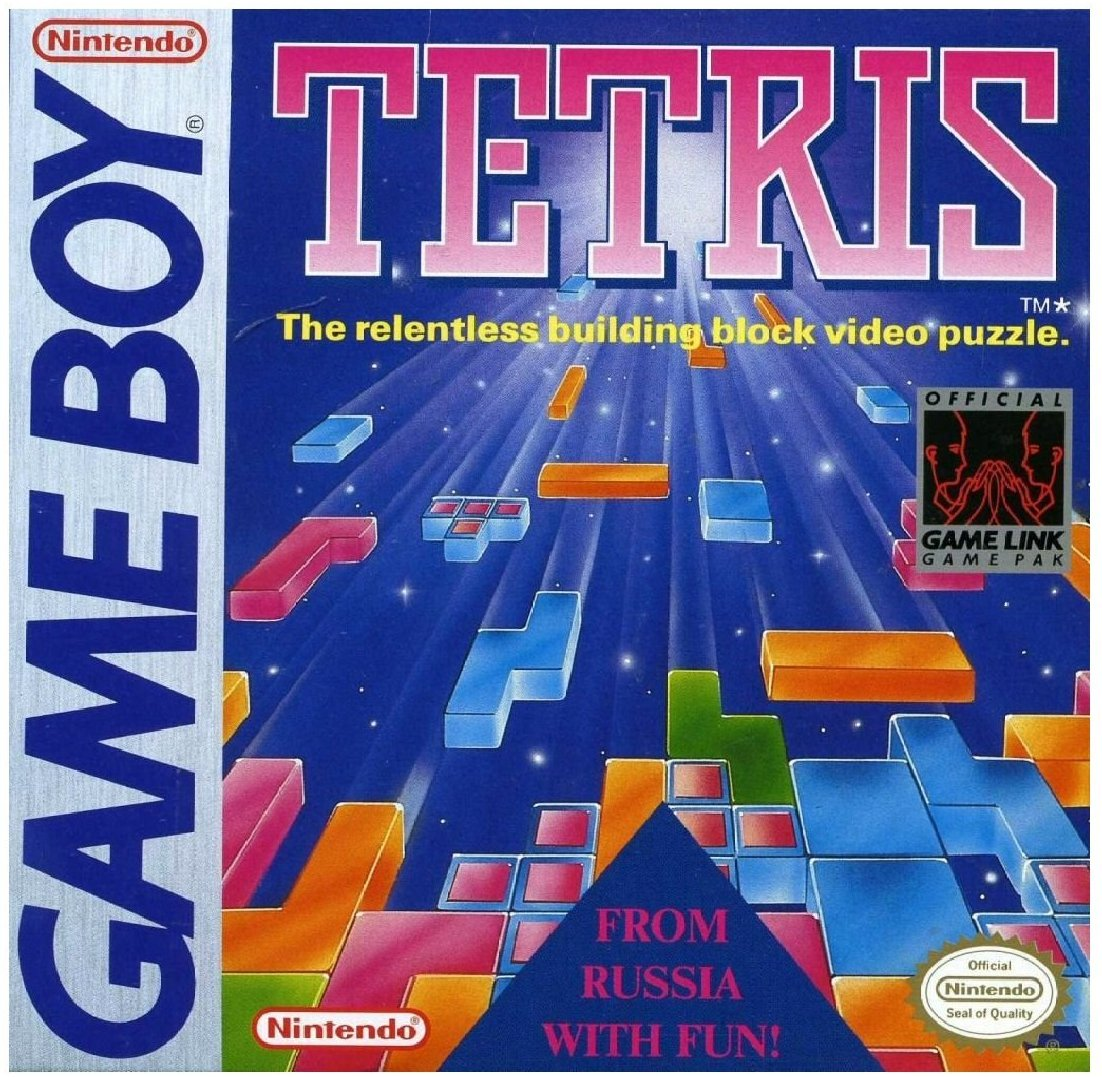
\includegraphics[width=.75\linewidth]{assets/assets/dmg-tr/dmg-tr-1.jpg}}\end{figure}\vspace{\baselineskip}
\begin{itemize}[left=0pt, nosep]
\item Japanese release in June 1989
\item Japanese release in June 1989
\begin{itemize}
\item Tsushin Cable Set
\end{itemize}
\item North American release in July 1989
\item Australian release in 1989
\item European release in September 1990
\item Asian release in 1990
\item Korean release in 1990
\item Brazilian release in 1993
\item North American release in May 1996
\begin{itemize}
\item Player’s Choice
\end{itemize}
\item Japanese release in September 2000
\begin{itemize}
\item Nintendo Power
\end{itemize}
\item Developed by Nintendo

\end{itemize}
\newpage\FloatBarrier\section*{Ecstasy of Order}
\begin{wrapfigure}{L}{0pt}{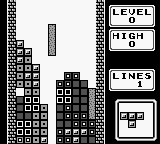
\includegraphics[width=.45\linewidth]{assets/assets/dmg-tr/dmg-tr-2.png}}\end{wrapfigure}\noindent
This is it. The game that single-handedly built the Game Boy as a viable, popular and beloved platform. Were Nintendo to have released the Game Boy with \emph{Tetris} stuck in the system unable to play anything else this brand new portable system would have been a tremendous success, making Nintendo a nice sum of money. Indeed, when we look at the Game Boy with modern eyes the system appears underwhelming. These days everybody carries a phone. They’re easy to put in your pocket or your purse. Their usefulness is also readily apparent. But how could you justify lugging such a big unwieldy brick around in the ’90s?\par
Because of \emph{Tetris}.\par
It might seem quaint in hindsight, but \emph{Tetris} in 1989 was revolutionary. Puzzle games existed but they were \emph{mostly} concerned with moving characters around mazes. \emph{Tetris} was different because it made you place falling objects. It was the first of its kind, and it resonated with people immediately. It is so simple I’ll summarize it in a single sentence for you: Make lines by placing the Tetrominos. If you don’t know what \emph{Tetris} is, go play it for a moment and you will immediately understand why so many people bought the Game Boy: the appeal of \emph{Tetris} was that strong.\par
\begin{quote}\emph{Tetris} made Game Boy and Game Boy made \emph{Tetris}.\newline \emph{ — Henk Rogers}\end{quote} \par
\FloatBarrier\section*{System Builder}
\emph{Tetris} is the game that built the Game Boy. Without it, the release of the system does not have a game of truly universal appeal. When the Game Boy was originally released, the presence of \emph{Tetris} on the system meant that business people, parents, children, basically anyone could enjoy the pea soup screen of the chunky Game Boy with an unparallelled experience. The main appeal of the revolutionary puzzle game, playing it in your palms, could not be achieved on any competitors’ machine since \emph{Tetris} was exclusive to portable consoles made by Nintendo. To the layman, \emph{Tetris} could even appear to have been invented by Nintendo. Except for the whole Russian theme the game has. While the match made in heaven was packed together in the same box in North America, Japan is a different story. \emph{Tetris} did not come out at the same time as the system in Japan. The Game Boy came out in April with \emph{Super Mario Land}, \emph{Alleyway}, \emph{Baseball} and \emph{Yakuman}, a mahjong title. \emph{Tetris} joined them two months later in June. I do not know exactly why that is, whether the game was simply not ready or something else more complicated. I tend to think it simply wasn’t finished in time because of the licensing history I’ll touch on later. \emph{Tetris} was thus not bundled with the Game Boy but keep in mind that the Japanese market very rarely bundles games with systems. It’s a matter of marketing tradition and consumer expectations. I don’t think it would have been bundled even if it came out at the same time as the Game Boy.\par
\begin{wrapfigure}{R}{0pt}{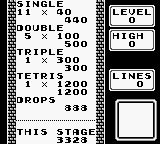
\includegraphics[width=.45\linewidth]{assets/assets/dmg-tr/dmg-tr-3.png}}\end{wrapfigure}
I absolutely need to clarify that \emph{Tetris} was not \emph{created} for the Game Boy, merely adapted. The long and sordid story of \emph{Tetris} leaving Motherland Russia and taking the rest of the world by storm is convoluted. Keeping it simple, Alexei Pajitnov created it in 1984 and it seeped to Europe and the rest of the West through home computer versions licensed and sub-licensed from the Soviet state. The British licensees got careless with their license, straight up acting like they owned the game, and licensed beyond what they had negotiated with the Soviets. Henk Rogers ended up with a Japanese video game console license that way. When he first saw the game, Hiroshi Yamauchi, Nintendo’s ruthless president, understood the match made in heaven between the upcoming Game Boy and \emph{Tetris}. He then had Henk Rogers sent on Nintendo’s behalf to negotiate for portable consoles terms. Henk Rogers, founder of Bullet-Proof Software, was a rare westerner working successfully in the Japanese game market (he famously introduced the Japanese to RPGs with \emph{The Black Onyx}) and he had come in contact with \emph{Tetris}, had fallen in love and started paying for a Japanese licence from the supposed British sub-licensee of Pajitnov, the game’s creator. He traveled to Moscow to make sure the game could be published on Game Boy and discovered that Elektronorgtechnica (ELORG), the Soviet organization that owned \emph{Tetris} because Pajitnov created the game at his job, had not licensed the game for console to anybody. Imagine that: Rogers was selling an illegal Famicom version according to the Soviets, and he learned it while trying to negotiate with them. Just as Henk had been able to get Yamauchi to trust him, he managed to convince the Soviets to trust him and he managed to secure a legitimate licence in 1989 from ELORG. He pissed off Atari in the process to the point where the fight between them and Nintendo over \emph{Tetris} eventually had to go to court, and through that whole process Rogers became a lifelong friend and business partner of Pajitnov to this day.\par
\FloatBarrier\section*{My Personal Affair With Tetris}
When I think of \emph{Tetris}, I hear the sounds you hear when you start a game. I don’t mean the specific music you hear when you play a game of \emph{Tetris}. I hear the bare minimum notes you need to hear on every screen before the game switches to the next one as you mash the A button. That’s how much I played \emph{Tetris}: enough to recall, 25 years after first playing it, the specific sounds it makes as you quickly start it up. I owned a Game Boy for two years with \emph{Tetris} as the only game. \textbf{And I loved it}. So when I say that \emph{Tetris} is the most important game on Game Boy, I’m talking from \textbf{experience}.\par
The game features two modes, aptly titled A-Type and B-Type. A-Type is strictly a top score type of deal. You can select how fast you want the game to start at, but this is it. B-Type tasks you with getting the highest score possible while clearing out a maximum of 25 lines. As a score multiplier, you can choose a speed setting and spew random blocks on the play field. While those two types of gameplay are awfully limited today (Nintendo’s last \emph{Tetris} version they developed themselves, \emph{Tetris DS}, features six very intricate modes), \emph{Tetris} set the standard for puzzle games for a decade. To top off this non-stop fun, the game features the same Russian-folklore stereotypes as all previous licensed versions of the game, including a rendition of folkloric Russian song \emph{Korobeiniki}, now better known for being the \emph{Tetris} \textbf{music} than for being a classical Russian song.\par
\FloatBarrier\vspace{\baselineskip}\begin{figure}[H]\centering{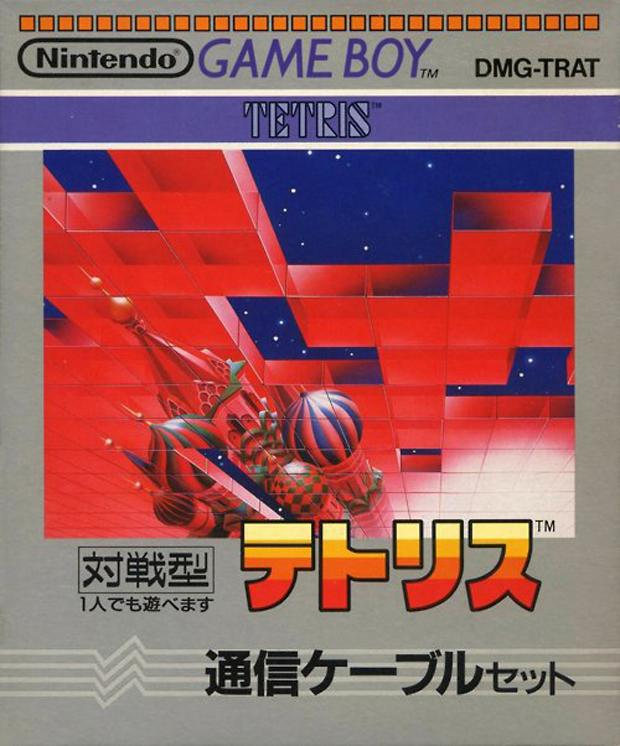
\includegraphics[width=.5\linewidth]{assets/assets/dmg-tr/dmg-tr-4.jpg}}\end{figure}
Weird fact, the first pressing of the Japanese version features some differences in the rule set and a different A song that isn’t \emph{Korobeiniki}. It’s still mind-boggling to me and probably explained by the fact that \emph{Korobeiniki} was first used on the Apple IIGS and Mac versions of \emph{Tetris} before Nintendo made their own. They probably later realized that \emph{Tetris} was already associated with the song and changed the A song for all subsequent pressings. It’s just a guess though.\par
\FloatBarrier\section*{Stronger Than Shigeru Miyamoto}
\begin{wrapfigure}{R}{0pt}{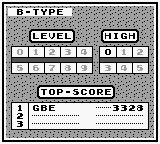
\includegraphics[width=.45\linewidth]{assets/assets/dmg-tr/dmg-tr-5.png}}\end{wrapfigure}
\emph{Tetris} on Game Boy is truly prescient. By merely bringing over the puzzle game to the Game Boy, Nintendo showed what it truly means to make a portable game. No need for Miyamoto to come in and invent what it means to make a game for Game Boy. The Famicom in Japan had very different games until Miyamoto came in and started literally expanding the boundaries of the console with games like \emph{Devil World}, \emph{Ice Climber} and, of course, \emph{Super Mario Bros.} Nowadays a new Nintendo console means a Miyamoto produced title like \emph{Super Mario~64}, \emph{Wii Sports}, or \emph{Steel Diver} will show everyone what the console is meant to do. The Game Boy did not see Miyamoto make a game for it until \emph{Wave Race} in 1992. Miyamoto is thus completely absent as the trendsetter of the Game Boy library. This impacts Nintendo’s first portable console \emph{from its first title to its last}. No other Nintendo console really had an absent Miyamoto, aside from the dreaded Virtual Boy. When he did show up with Game Boy games, he was the one who had to follow suit, not the other way around. In the end, the Game Boy is the only Nintendo console with Miyamoto being a minor influence.\par
\FloatBarrier\section*{Saving}
Since \emph{Tetris} is a game where you are challenging yourself to become better at playing it, turning it off is of no concern. Even if your bus has arrived, if your meeting starts soon or if your batteries have run out, you can turn off the Game Boy without a second thought. It’s the perfect portable game because any progress you make playing it is not kept in the cartridge, it’s kept inside \textbf{you}. There’s always the next game, where you can keep honing your skills. That’s the whole point of the game: getting better at \emph{Tetris}.\par
The game is not without its quirks. It has a beautiful and prominent score board, but there’s no battery in the cartridge to keep your score if you turn off your Game Boy. Why show your best score \textbf{and have you spend so much time inputting your initials} if you’re not going to keep it? This is utterly pointless. \emph{Tetris~DX}, released along with the Game Boy Color years later will solve that weird misstep.\par
\FloatBarrier\section*{Playing With a Friend?}
We need to talk about the multiplayer. \emph{Tetris} was able to be a multiplayer success because \textbf{everybody} owned it, everybody liked it and every original Game Boy came with a link cable. Keep in mind, to play any link cable game on Game Boy, you need two copies of the game. \emph{Tetris} was ubiquitous, since it came with the system in North America and Europe. Since everyone owned it, it could easily be played with a friend. No other early Game Boy title can lay claim to be a multiplayer success. There were too many titles, too few copies lying around. \textbf{Until \emph{Pokémon} took over the world in 1998}. In retrospect, I feel that 95\% of all successful link cable connections were either \emph{Pokémon} trades or \emph{Tetris} games.\par
\emph{Tetris} thus showed the possibilities of playing a game with a friend who was looking at his own screen. It was a beautifully designed multiplayer experience that made the Game Boy shine, but it did not birth a vibrant crop of link cable titles for Game Boy. In hindsight, the Game Boy was a multiplayer failure until \emph{Pokémon}. The release of the pocket monster game will radically redefine the Game Boy. Until 1998, Game Boy \& \emph{Tetris} were synonymous, in multiplayer and in the public’s consciousness. But once \emph{Pokémon} arrives the Game Boy will gain a second wind, a feat no other console ever managed. Hardware sales will pick up and massively increase after years of moribund numbers. Such is the strength of Pokémon: \emph{Gotta Catch ’Em All} sold Game Boys!\par
\FloatBarrier\section*{Conclusion}
\emph{Tetris} truly showed how to do it right on a system that was the first of its kind. While the system was not under-powered, the true bottleneck in terms of design was the screen. Unlit, pea soup green, and with ghosting issues. \emph{Tetris} is essential because it showed how to properly use the limited screen of the Game Boy. Non-intricate backgrounds to help with the limited colour palette, large elements who move slowly to help with ghosting. Great Game Boy games would take those lessons to heart and try not to cram complicated console graphics on the tiny screen.\par
\textbf{AND} it’s essential because it was a runaway mainstream success whose influence is still felt today.\par
\FloatBarrier\vspace{\baselineskip}\begin{figure}[H]\centering{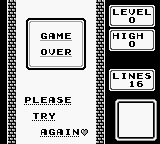
\includegraphics[width=4.85cm]{assets/assets/dmg-tr/dmg-tr-6.png}}\end{figure}
\chapter*{Heroes of Might \& Magic}\markboth{Heroes of Might \& Magic}{}\addcontentsline{toc}{chapter}{Heroes of Might \& Magic}
\vspace{\baselineskip}\begin{figure}[H]{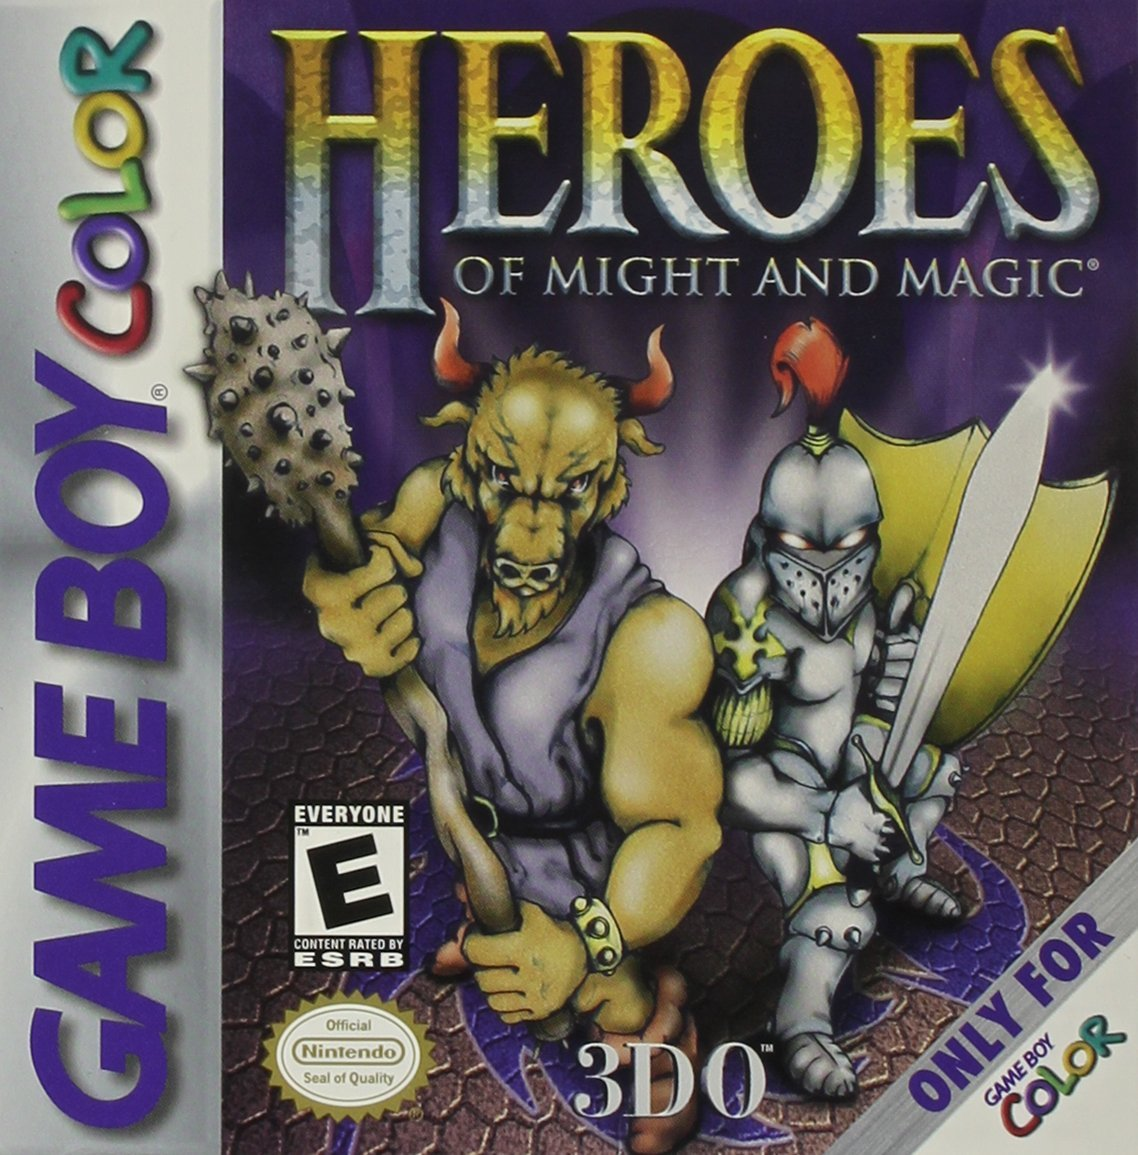
\includegraphics[width=.75\linewidth]{assets/assets/cgb-auhe/cgb-auhe-1.jpg}}\end{figure}\vspace{\baselineskip}
\begin{itemize}[left=0pt, nosep]
\item North American release in June 2000
\item European release in October 2000
\item Never released in Japan
\item Developed by KnowWonder

\end{itemize}
\newpage\FloatBarrier\section*{Buy, Move, Attack, Rinse, Repeat}
\begin{wrapfigure}{L}{0pt}{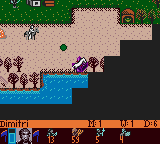
\includegraphics[width=.45\linewidth]{assets/assets/cgb-auhe/cgb-auhe-2.png}}\end{wrapfigure}\noindent
\emph{Heroes of Might \& Magic} is the textbook example of what Game Boy Essentials is about. If you look at lists of \textbf{best Game Boy games of all time}, that game will \textbf{never} be on there. But it is \textbf{very} essential to play \emph{Heroes of Might \& Magic} to understand a small part of the Game Boy Color’s library: the \textbf{let’s do something you didn’t think could be done} type of games. Games like \emph{Warlocked}, \emph{Alone in the Dark} or the unreleased \emph{Tyrannosaurus Tex} were all trying to cram Real-Time Strategy, Third Person Horror or First Person Shooter gameplay on Game Boy Color with limited success. Also of note is the unreleased \emph{Katakis 3D}, an ambitious space shooter that was recently unearthed. \emph{Heroes of Might \& Magic} was part of that overall trend happening near the end of the Game Boy Color’s life. Mind you, it was never what was popular or the point of the machine; the \emph{Pokémon} clones and media property tie-in games were what was prevalent at the time. And they weren’t the best games either: the best games on the system were never those games who broke the mould of what should be done on an unlit portable system. The best games understood the limitation of the Game Boy. But games pushing the envelope were omnipresent in the last years of the Game Boy Color and gave more life to a system that was in all honesty running out of creative juices. \textbf{And I loved those efforts}. When I was a fourteen year-old kid in 2000, I was fascinated by those types of games. I was genuinely \textbf{excited} for \emph{Tyrannosaurus Tex} and the port of the first \emph{Resident Evil}, two unfinished games who left me yearning for more. So I enjoy looking at the brethren of those games again with fifteen years of insight.\par
Now that we have set \emph{Heroes of Might \& Magic} in context, let’s talk about what the game is. \emph{Heroes of Might \& Magic} is a port of a classic pseudo-RTS PC game. You get a castle and an army, you fill up the army with units bought from the castle while exploring the map. Exploring allows you to find treasures and resources to help you out. Finally, you fight other armies on a battle screen; a hexagonal grid where all your individual units are stacked, severely limiting the tactical possibilities.\par
\begin{wrapfigure}{R}{0pt}{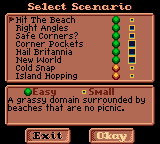
\includegraphics[width=.45\linewidth]{assets/assets/cgb-auhe/cgb-auhe-3.png}}\end{wrapfigure}
\emph{Heroes of Might \& Magic} is not too complicated without a keyboard and mouse. Even though it’s originally a PC game, the game’s interface is workable if convoluted. It uses A/B to confirm/cancel, with the Select button holding the ability to switch between towns or heroes. So it’s that weird kind of game where you’ll be pressing Select a whole bunch. The game is also buggy. I had to stop playing the game because the AI kept casting Berzerker on my multi-headed snakes; this caused them to get stuck in an endless animation loop, preventing me from progressing further in the game. In all honesty, I was kind of relieved to get an excuse to stop playing.\par
\FloatBarrier\vspace{\baselineskip}\begin{figure}[H]\centering{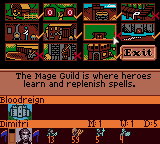
\includegraphics[width=4.85cm]{assets/assets/cgb-auhe/cgb-auhe-4.png}}\caption*{There is neither campaign mode, nor multiplayer. The only things available to play are skirmish maps. You don’t even get to choose your starting race.}\end{figure}
Strategies are inexistent. You don’t really even need to limit what you buy, since you easily get enough cash every week to buy everything you need. The heroes’ placement is ultimately irrelevant, since the maps are so big. Five units on a ginormous map can’t properly convey strategies. Your heroes just find one another, and attack one another. That’s it. When they attack one another, the hexagonal grid fighting strategy is way less complex than it should. Mostly because the game stacks your units. You can’t bring more than five different types of units with your army, and there are harsh limits on the number of heroes you can have in the field. What invariably happens is that you then build one gigantic army that moves around all over the map, steamrolling without any strategy every goon placed on the map in front of the treasures. That’s all fine and good, but you’ll be spending most of your time playing that game just shuffling units from your town to that army. It’s spring-cleaning video gaming.\par
\begin{wrapfigure}{L}{0pt}{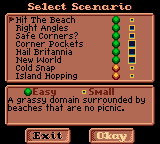
\includegraphics[width=.45\linewidth]{assets/assets/cgb-auhe/cgb-auhe-5.png}}\end{wrapfigure}\noindent
I liked \emph{Heroes of Might \& Magic 3} on PC having played it hot-seat multiplayer with friends. Its mechanics lends itself well to a co-op game. It is a fun experience playing turn-by-turn with a beer while having a chat, even with all its anemic strategy. You’ll accept a lot of bullshit when playing with a friend. The Game Boy could have recreated that nice, no frills experience with a nice hot-seat multiplayer mode. It would have been perfectly suited to play that game with a friend. You would just take turns holding the console. Instead the game has \textbf{no} multiplayer of any kind. Your only option is playing against the AI in skirmish maps. No campaign, no multiplayer, no choosing your starting race even. Symptoms of an unfinished game.\par
Which brings me to my main point of contention with the game. Play it long enough (and when I mean long enough, I mean more than an hour) and you’ll bump into one of the Game Boy Color’s flaw: it can’t really do artificial intelligence. As much as this game’s gameplay is not conducive of any strategy, it does not matter. All the CPU does is move back and forth, barely buying any units, waiting to be trounced by your armies. There’s no challenge to this game, even on the supposedly \emph{hard} maps. Most other Game Boy Color games hide their non-existent AI behind the mechanics of their game. \emph{Heroes of Might \& Magic}, being a port of a PC game, gets no such luxury. Every aspect of the game could be kind-of ported to the GBC, except the AI.\par
\begin{wrapfigure}{R}{0pt}{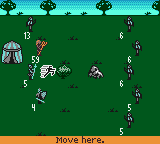
\includegraphics[width=.45\linewidth]{assets/assets/cgb-auhe/cgb-auhe-6.png}}\end{wrapfigure}
There is maybe one hope in terms of AI: the Game Boy War games. Made by Nintendo, and known here as the \emph{Advance Wars} series, the games started on the Famicom and moved to Game Boy from there but were never released outside Japan until the GBA games. They are fun, simple turn-based strategy games that hide their shortcomings very well. I have yet to play any of the Japan-only \emph{GB Wars} games, and look forward to see if they have a reasonable difficulty curve and an interesting AI.\par
\FloatBarrier\section*{Conclusion}
\emph{Heroes of Might \& Magic} has many faults, with the weakness of the AI and the absence of hot-seat multiplayer being fatal to making the game any good. It is essential because of how apparent those shortcomings are and because it was published in its unfinished state anyway.\par
\chapter*{Donkey Kong Land}\markboth{Donkey Kong Land}{}\addcontentsline{toc}{chapter}{Donkey Kong Land}
\vspace{\baselineskip}\begin{figure}[H]{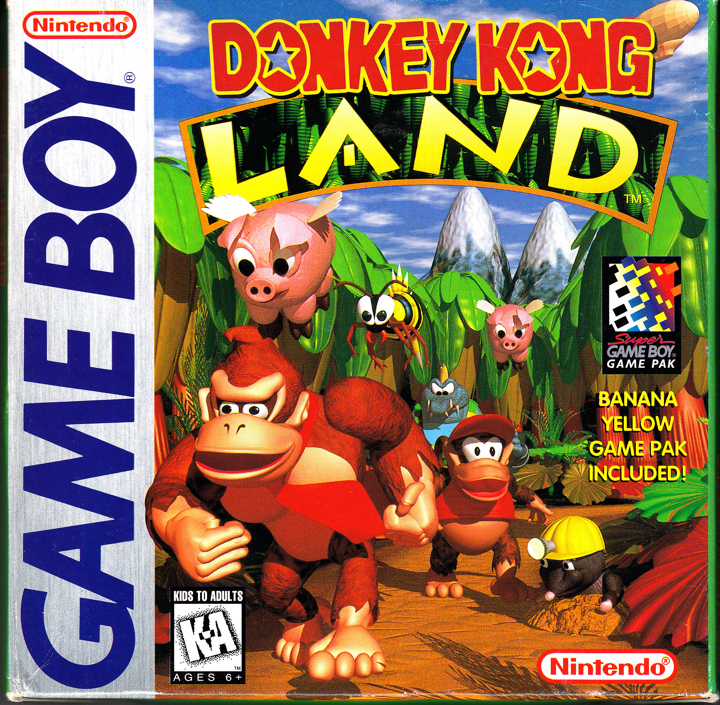
\includegraphics[width=.75\linewidth]{assets/assets/dmg-yt/dmg-yt-1.jpg}}\end{figure}\vspace{\baselineskip}
\begin{itemize}[left=0pt, nosep]
\item North American release in June 1995
\item Japanese release in July 1995
\item European release in August 1995
\item North American release in 1997
\begin{itemize}
\item Player’s Choice
\end{itemize}
\item European release in 1997
\begin{itemize}
\item Nintendo Classics
\end{itemize}
\item North American release in November 1999
\begin{itemize}
\item Player’s Choice Re-release
\end{itemize}
\item Japanese release in March 2000
\begin{itemize}
\item Nintendo Power
\end{itemize}
\item Developed by Rare Ltd.

\end{itemize}
\newpage\FloatBarrier\section*{Monkeying Around}
\begin{wrapfigure}{L}{0pt}{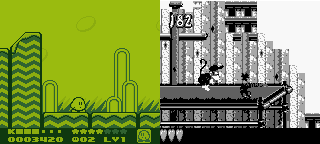
\includegraphics[width=.45\linewidth]{assets/assets/dmg-yt/dmg-yt-2.png}}\end{wrapfigure}\noindent
\emph{Donkey Kong Land} is the worst case scenario. All the mistakes a team can make when adapting a concept to Game Boy, they’re all there. Dark backgrounds? Check. Overtly busy sprites? Check. Leaps of faith level design? Check. Poor physics? Check. If you want to know how not to make a Game Boy game, look no further, this game has done everything wrong!\par
With their SNES game, Rare was able to convince everyone that a polygonal game was running on the humble Super Nintendo hardware. With the Game Boy adaptation, they revealed their monkey antics. LOL.\par
I got \emph{Donkey Kong Land} in 1995 when it was released, so it’s one of those games where I’m super critical because \textbf{I’ve owned it for 20 years}. When I was a kid, it took me days to understand what the KONG letters you collected were supposed to be. Not as a concept, I mean as an object. I didn’t know what those squares were! Were they TVs? Candy? I couldn’t decipher them. Why? Because the game is simply too hard to see on an original Game Boy. I really love the SNES \emph{Donkey Kong Country} games. \emph{DKC~2} is up there in the pantheon of eternal games. The \emph{Donkey Kong Land} sub-series, not so much.\par
But people \textbf{love} this game. To those people I must say I’m sorry, I kind of liked it when I was a kid despite its flaws but the only thing essential about \emph{Donkey Kong Land} is its myriad of flaws. They paint a much more interesting portrait than the few things it did right.\par
\FloatBarrier\section*{Forgetting About the Ghosts in the Machine}
Let’s talk about \emph{Donkey Kong Land} by discussing first what it was displayed on, the Game Boy screen. The shortcomings of the screen usually talked about are:\par
\begin{itemize}

\item It’s unlit;
\item It’s only four shades of grey with a pea-soup green background.

\end{itemize}
\begin{wrapfigure}{R}{0pt}{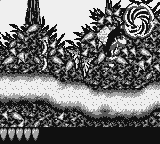
\includegraphics[width=.45\linewidth]{assets/assets/dmg-yt/dmg-yt-3.png}}\end{wrapfigure}
But people always forget about a last shortcoming: the screen suffers from severe ghosting. What is ghosting? It’s a slow time to turn off a pixel when it was displaying colour before. When the Game Boy tells its screen to turn a pixel off, if the screen is displaying an exploding bomb for example, then the time to turn off that pixel is not instantaneous. So when a character is moving, as is the case with \emph{Super Mario Land} for example, he leaves a trail of blurry pixels behind. That’s fine for Mario because he is small, surrounded by pixels turned off and you’re moving in a single direction, so that leaves a trail \textbf{behind} him. When he gets near an enemy or a wall, anything that produces ghosting of its own, the whitespace allows you to keep making sense of what’s on the screen. So it’s never too much of an issue.\par
At this point remember that no screenshot I can show you can display the ghosting the Game Boy’s screen suffers. It’s a result of movement, and you can only see that movement artifact on an original screen. My screenshots serve only to show what Rare \textbf{didn’t do} to alleviate the problem.\par
You might be tempted to think that only characters can cause ghosting, but everything that moves on the screen does. So when you move forward, or jump, or swim, or swing on vines the Kongs, enemies, platforms, background elements, barrels, bananas, basically everything clashes with everything else. This causes general ghosting and turns the screen into a mess of late pixels trying to catch up to a game too complicated for the puny screen: everything’s blurry. The processor and the graphics chip are fine, mind you, the game suffering no slowdown at all. It’s the screen who never catches a break. Any moving thing will create ghosting. Thus, you have to be careful when creating a game’s environment to keep it simple. To show you what I mean, let’s compare two games released around the same time:\par
\FloatBarrier\vspace{\baselineskip}\begin{figure}[H]\centering{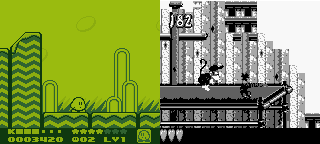
\includegraphics[width=.6\linewidth]{assets/assets/dmg-yt/dmg-yt-4.png}}\caption*{\emph{Kirby’s Dream Land~2} and \emph{Donkey Kong Land}.}\end{figure}
On the one hand, \emph{Kirby} uses its art style and restraint to show a vibrant, dare I say colourful world while keeping a healthy dose of whitespace to keep the ghosting out of the way. Objects have shapes, but are not coloured when you can move in front of them. They have borders, but not patterns. I’ll grant you that the grass is borderline, but there the game relies on Kirby’s whiteness to prevent an excess of ghosting. Truly great developers like HAL Laboratory knew how to push the limits of a piece of hardware, but \textbf{not exceed those limits}. \emph{Donkey Kong Land}, on the other hand, is not Rare at its best. This is the worst of early 80s Rare. When they made dubious games for ZX Spectrum. It has no sprite borders and a busy background and is thus a blurry indecipherable mess.\par
If you look at a picture of the game, you’ll see what I mean when I talk about an undecipherable mess. It takes you an extra moment to process what you’re looking at. Observe carefully a screenshot of \emph{Donkey Kong Land} and think on what your brain has to do to decipher what you’re looking at. I don’t know about you, but I can feel the gears turning in my head trying to understand what’s happening and that’s without ghosting. Now imagine that everything is moving at 59.7 frames a second and blurry. And green.\par
\FloatBarrier\vspace{\baselineskip}\begin{figure}[H]\centering{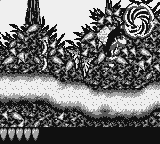
\includegraphics[width=4.85cm]{assets/assets/dmg-yt/dmg-yt-5.png}}\caption*{Can you spot Donkey Kong in that picture? Now try it on a Game Boy screen.}\end{figure}
You might argue that the game features different environments and that we should also look at the other type of backgrounds. You are correct. The first set of levels uses the jungle tileset, the worst of the whole game in terms of readability, but believe me the others are not much better. Why? Because there still is no respect for what the screen can’t do right. See for yourself.\par
\FloatBarrier\vspace{\baselineskip}\centering
\begin{minipage}{0.45\linewidth}\adjustbox{valign=t}{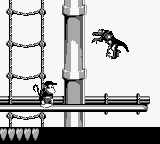
\includegraphics[width=\linewidth]{assets/assets/dmg-yt/dmg-yt-6.png}}\end{minipage}\vspace{2pt}
\begin{minipage}{0.45\linewidth}\adjustbox{valign=t}{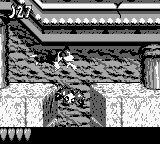
\includegraphics[width=\linewidth]{assets/assets/dmg-yt/dmg-yt-7.png}}\end{minipage}\vspace{2pt}
\begin{minipage}{0.45\linewidth}\adjustbox{valign=t}{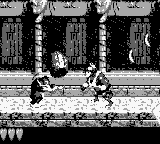
\includegraphics[width=\linewidth]{assets/assets/dmg-yt/dmg-yt-8.png}}\end{minipage}\vspace{2pt}
\begin{minipage}{0.45\linewidth}\adjustbox{valign=t}{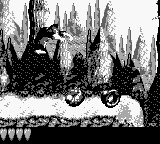
\includegraphics[width=\linewidth]{assets/assets/dmg-yt/dmg-yt-9.png}}\end{minipage}\vspace{2pt}
\begin{minipage}{0.45\linewidth}\adjustbox{valign=t}{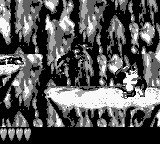
\includegraphics[width=\linewidth]{assets/assets/dmg-yt/dmg-yt-10.png}}\end{minipage}\vspace{2pt}
\begin{minipage}{0.45\linewidth}\adjustbox{valign=t}{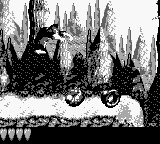
\includegraphics[width=\linewidth]{assets/assets/dmg-yt/dmg-yt-11.png}}\end{minipage}\vspace{2pt}
\begin{minipage}{0.45\linewidth}\adjustbox{valign=t}{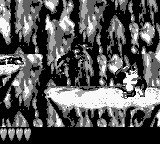
\includegraphics[width=\linewidth]{assets/assets/dmg-yt/dmg-yt-12.png}}\end{minipage}\vspace{2pt}
\begin{minipage}{0.45\linewidth}\adjustbox{valign=t}{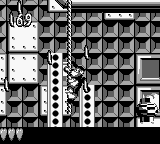
\includegraphics[width=\linewidth]{assets/assets/dmg-yt/dmg-yt-13.png}}\end{minipage}\vspace{2pt}
\begin{minipage}{0.45\linewidth}\adjustbox{valign=t}{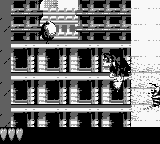
\includegraphics[width=\linewidth]{assets/assets/dmg-yt/dmg-yt-14.png}}\end{minipage}\vspace{2pt}
\begin{minipage}{0.45\linewidth}\adjustbox{valign=t}{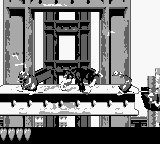
\includegraphics[width=\linewidth]{assets/assets/dmg-yt/dmg-yt-15.png}}\end{minipage}\vspace{2pt}
\begin{minipage}{0.45\linewidth}\adjustbox{valign=t}{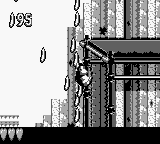
\includegraphics[width=\linewidth]{assets/assets/dmg-yt/dmg-yt-16.png}}\end{minipage}\vspace{2pt}
\begin{minipage}{0.45\linewidth}\adjustbox{valign=t}{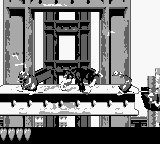
\includegraphics[width=\linewidth]{assets/assets/dmg-yt/dmg-yt-17.png}}\end{minipage}
\par\justifying
You have some breaths of fresh air in there but most of the game’s art style is simply too complicated for Game Boy. Now that we’ve completely tarnished the game’s art style, I feel I need to remind you I love Rare’s \emph{Donkey Kong} games on SNES. A very appropriate art style of pre-rendered graphics for a system that could handle the load. Unless your TV was somehow a Game Boy screen. But I digress.\par
There is another thing we need to talk about that induces ghosting: the camera. In a 2D side-scrolling game, you need to build a movement system for the camera. You cannot just directly map camera movement to character movement. Play \emph{Super Mario Bros.} and look at how the camera establishes boxes for Mario to decide whether the screen will move or not. I could go into detail about how the boxes in \emph{Donkey Kong Land} work but suffice it to say they’re all screwed up! I can talk of one telling example.\par

There is an unnecessary camera move upward when jumping while standing still. It is one of the many ways the camera causes undue ghosting. Other games will prefer large, generous camera boxes that will allow you to reach nearly to the top of the screen before scrolling. It’s a choice with consequences (you can see less of what’s above you) but Rare chose the wrong priority here.\par
\FloatBarrier\section*{Bad Intentions}
So what were the intentions of Rare with \emph{Donkey Kong Land}? Obviously, they were on a mission to bring the CGI graphics of \emph{Donkey Kong Country}, the revolutionary SNES game from 1994, on the tiny Game Boy. They did, but was it worth it? When it was released, \emph{Donkey Kong Country} was a revelation. \textbf{You can do 3D graphics on Super Nintendo?} Of course the answer is they couldn’t. They faked it by building 3D models of everything on Silicon Graphics workstations. The developers at Rare then turned pictures of those 3D graphics into 2D sprites and tiles that worked on the SNES. When they planned and built a Game Boy version of \emph{Donkey Kong Country}, they said, “let’s do the same thing!”\par
\FloatBarrier\vspace{\baselineskip}\begin{figure}[H]\centering{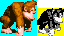
\includegraphics[width=.6\linewidth]{assets/assets/dmg-yt/dmg-yt-19.png}}\caption*{Super Nintendo original next to the Game Boy bastard child.}\end{figure}
You can see how the sprite of the Game Boy version is similar to the Super Nintendo original. They obviously started from those same 3D models built on SGI workstations and ran them through a process that made them into Game Boy sprites. While I would argue the final sprites on SNES are a \emph{tour de force}, the GB sprites are a step backward. A technological process whose final result is not as good as giving every sprite a hand-drawn border. Keep in mind I’m showing you the best result of this process; the character of Donkey Kong, who was certainly given the most scrutiny. I’ve already talked about how bad the result were with the background tiles.\par
I’ll quickly address one other issue: screen crunch. A common complaint against \emph{Donkey Kong Land} is that the sprites are too big for the tinier screen of the Game Boy. Well, the SNES has a 256 pixels horizontal resolution. The Game Boy? 160 pixels. Donkey Kong on SNES is 40 pixels wide, so to be the same proportions he should be 25 pixels wide. DK on Game Boy is 27 pixels wide. So no, the sprites are not too big. They’re similar in proportions. Rare made all the sprites size appropriate. However, when people complain about the size of the sprites they are simply pointing the finger at the wrong culprit. You see, like we discussed earlier, Rare messed up the camera system. Donkey and Diddy end up in the middle of the screen when moving or even worse, on the right side of the screen when rolling. So you never see what’s coming. You end up having to make tons of leaps of faith, not knowing if there is something on the other end of your jump, and when you’re running or rolling you have no reaction time. Your nose is too close to the action even with size appropriate sprites. \emph{Donkey Kong Country} on SNES had no such problems.\par
\FloatBarrier\vspace{\baselineskip}\begin{figure}[H]\centering{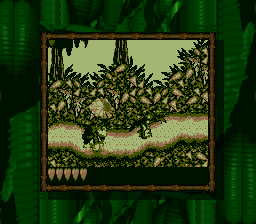
\includegraphics[width=.6\linewidth]{assets/assets/dmg-yt/dmg-yt-20.png}}\end{figure}
\FloatBarrier\section*{A Game for Super Game Boy Perhaps?}
I cannot shake from my mind the idea that after looking at all of these quirks and faults that the game was built primarily for the Super Game Boy. I do not know how development kits for the Game Boy worked in 1995, but I would bet money most testing was done on the Super Game Boy, not the original Game Boy. There’s no ghosting and the colour helps with the characters and background. But even with the Super Game Boy they bungled it. Read Christine Love’s article on \emph{Donkey Kong} and \emph{Donkey Kong Land} to see how even if they \emph{might} have built the game with the Super Game Boy, they didn’t do anything right.\par
\FloatBarrier\section*{Saving}
In my Tetris article, I talked about how important it is that Tetris features no saving but all the progress is in you, and how that is super cool. In \emph{Donkey Kong Land}, you can’t save the game unless you gather all the KONG letters in a level. You want to save, you’d better get through a level you know well and find all those goddamn letters without losing all your lives. It’s super dumb and unfair. \textbf{If the game was a masterpiece, this would be a travesty worth decrying.} Here, because everything else is so wrong, I just mention it and move on.\par
\FloatBarrier\section*{The Music}
Let’s end this on a good note. Graeme Norgate and Dave Wise made very good music for that game. They mostly use the soundtrack of \emph{DKC} as a springboard to do something different that recalls the original tracks. I like it. I was playing \emph{DKL} on my AGS-101 and found the music lovely. Then I switched to my original Game Boy and realized how finely tuned the music was to the speaker of the DMG-001. It’s good work worth mentioning. It really comes alive on original hardware.\par
\FloatBarrier\section*{Conclusion}
I’m sorry if you liked \emph{Donkey Kong Land} as a kid. I don’t know what kind of eyesight you have but I couldn’t see squat back then and I can’t see squat today. That’s why it’s essential. It’s what not to do when adapting a concept to Game Boy.\par
\chapter*{Yars’ Revenge}\markboth{Yars’ Revenge}{}\addcontentsline{toc}{chapter}{Yars’ Revenge}
\vspace{\baselineskip}\begin{figure}[H]{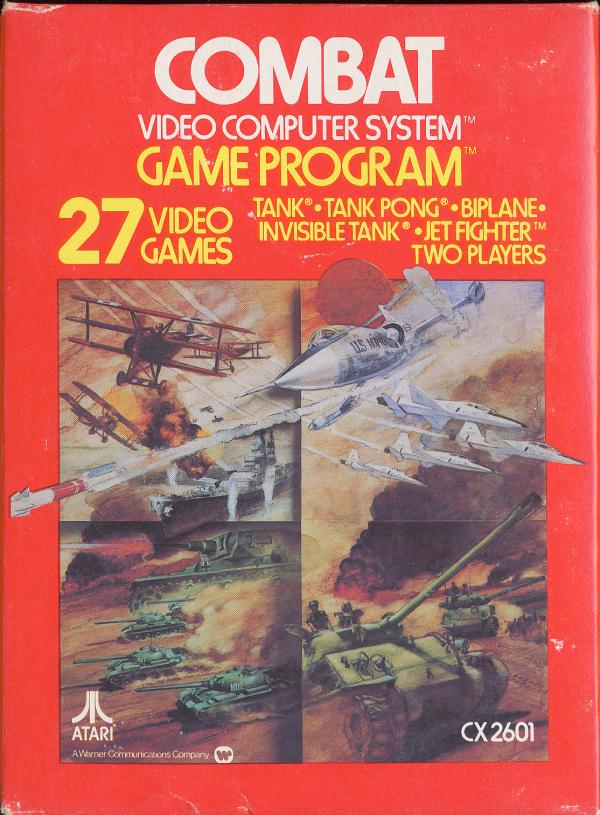
\includegraphics[width=.75\linewidth]{assets/assets/dmg-ayve/dmg-ayve-1.jpg}}\end{figure}\vspace{\baselineskip}
\begin{itemize}[left=0pt, nosep]
\item North American release in September 1999
\item European release in 2000
\item Never released in Japan
\item Developed by Telegames

\end{itemize}
\newpage\FloatBarrier\section*{A One-man Show From a Different Age}
\begin{wrapfigure}{L}{0pt}{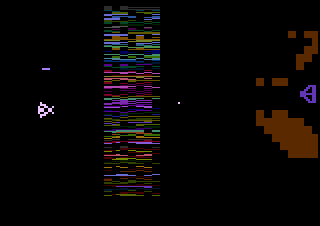
\includegraphics[width=.45\linewidth]{assets/assets/dmg-ayve/dmg-ayve-2.png}}\end{wrapfigure}\noindent
I love sitting down on the couch, taking out my binders full of Game Boy cartridges and looking at the games I have, trying to pick something to play. You usually never play only one game in a single sitting; you instead go from one game to the other, indulging in different styles of games throughout your play session. \emph{Yars’ Revenge} is the essential game to play between two bigger, more impressive games.\par
\FloatBarrier\section*{128 Bytes of Fun}
\emph{Yars’ Revenge} is the adaptation of an Atari VCS game released in 1982. Today, what is colloquially called the Atari is usually referred to as the Atari~2600. This is a second name given to the system in 1982 when its successor, the Atari~5200, was released. I personally prefer and use the original ’70s name: Atari Video Computer System. So nondescript.\par
On Game Boy Essentials, we talk about old games; \emph{Yars’ Revenge} is \textbf{old} old. So old, the original \emph{Yars’ Revenge} came out in what is usually called the \emph{golden age} of video game development. Why? Games were completely made by one person, working alone with next to no supervision. \emph{Yars’} was literally made by one man; an employee of Atari, Howard Scott Warshaw. Warshaw made three games and three games only: \emph{Yars’ Revenge}, \emph{Raiders of the Lost Ark} and \emph{E.T. the Extraterrestrial}. I know of no other programmer who can say they coded three games all on their own (Warshaw got artwork help for \emph{E.T.} though but I think we can forgive him for that one) and they all sold more than a million copies. I’d say he quit while he was ahead but his last game is \emph{E.T.} so, you know.\par
\begin{wrapfigure}{R}{0pt}{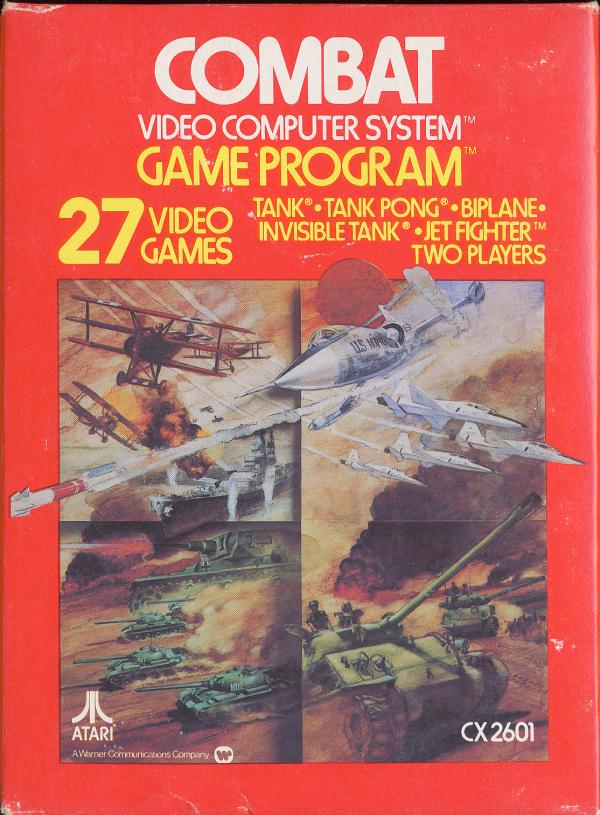
\includegraphics[width=.45\linewidth]{assets/assets/dmg-ayve/dmg-ayve-3.jpg}}\end{wrapfigure}
Anyway, \emph{Yars’ Revenge}, Warshaw’s first game is a seminal classic for the Atari and is a great representation of its era of Atari VCS development. Gone were the early days in 1977 of catch all titles like \emph{Combat} who proudly proclaimed to be 27 games in one. \emph{Yars’ Revenge} was a one-trick pony, but a \textbf{good} one. If you can figure out how it works.\par
\FloatBarrier\section*{Atari: Fun When You Figure It Out}
When I was a kid, I didn’t grok \emph{Yars’ Revenge}. I was around 6 or 7 and I remember going to a friend’s house who had an Atari VCS stashed high up in a closet. This wood-panelled box of mystery was too interesting not to play. Plus, there was a box full of games with it! We’d get it, spend an eternity trying to figure how to plug it in and try all the cartridges. \emph{Yars’ Revenge} was one of those games, and we just never figured out how it worked. We just played \emph{The Empire Strikes Back} instead. That one was easier to figure out. My point is simple: \emph{Yars’ Revenge} is not exactly self-explanatory if you don’t have the manual.\par
\FloatBarrier\section*{How to Play Yars’ Revenge}
You are Yar, an insect tasked with destroying the Qotile (I know, it sounds stupid to me too) who moves up and down along the right side of the screen. The Qotile is a triangle that can do one thing: it sometimes turns into a whirlwind and lunges at you, trying to kill you. It then leaves the screen and reappears in its spot. The Qotile is surrounded by an orange shield that protects it. You can shoot a little bullet to destroy the shield piece by piece, but no matter what you do, your little bullet cannot harm the Qotile. To destroy it, you need to charge up your Zorlon Cannon (ridiculous names is one of the downsides of single person development) by eating pieces of the orange shield or touching the Qotile when it isn’t a whirlwind. This goes against every gaming reflex I have but you do have to touch the main enemy of the game to ultimately kill it. The cannon then shows up on the left side of the screen and you then need to aim it (it stays on the same axis as Yar) at the moving Qotile and fire it. If you lined up everything just right, boom!\par
\FloatBarrier\vspace{\baselineskip}\begin{figure}[H]\centering{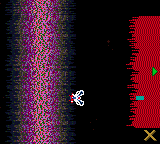
\includegraphics[width=.6\linewidth]{assets/assets/dmg-ayve/dmg-ayve-4.png}}\caption*{Interestingly, this is a composited screenshot I got from Wikipedia. The game seems to flicker between elements so no legitimate screenshot can show all the elements of the game.}\end{figure}
On top of that craziness, there’s the missile, relentlessly pursuing you. It’s not so much a missile as a silent rectangle stalker. It will constantly move in your direction, following you wherever you go; if you touch it, you’re dead. In the middle of the play field you have a safe zone where the missile will still pursue you but cannot kill you. That safe zone is a thing of beauty, built from a random block of the console’s RAM, constantly changing in random patterns. It’s coding gibberish turned into graphics. The VCS at its best.\par
When you clear a level it starts all over again with a different shield pattern and a faster missile and whirlwind. Repeat until you’re tired of playing it and want to play \emph{Save Mary} instead.\par
\FloatBarrier\section*{Let’s Put It on Game Boy!}
Let’s be clear here: \emph{Yars’ Revenge} on Game Boy is not a shining diamond illuminating the Game Boy library. It’s just an Atari classic that sold like gangbusters in its time, somewhat adapted for Game Boy. How?\par
\FloatBarrier\vspace{\baselineskip}\centering
\begin{minipage}{0.45\linewidth}\adjustbox{valign=t}{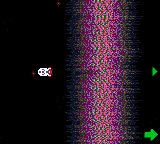
\includegraphics[width=\linewidth]{assets/assets/dmg-ayve/dmg-ayve-5.png}}\end{minipage}\vspace{2pt}
\begin{minipage}{0.45\linewidth}\adjustbox{valign=t}{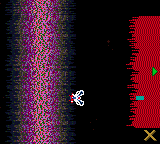
\includegraphics[width=\linewidth]{assets/assets/dmg-ayve/dmg-ayve-6.png}}\end{minipage}
\par\justifying
The most important consideration is a set of two glyphs on the right side of the screen. An arrow shows you where the Qotile is at all times, also warning you when a whirlwind is charging up. Since the play field is the same relative size as on the Atari, and the resolution is smaller, you need the arrow to keep you posted on where the Qotile is. It works surprisingly well.\par
On the bottom right of the screen, an arrow and X sign tells you what you need to do next. Go right to charge your Zorlon Cannon with the shield, now go left to arm it. Yeah, you need to go to the left side of the screen to \emph{arm} your weapon; this is how modes~6 and 7 of the original game, affectionately called in the manual \textbf{Ultimate Yars}, worked. The cannon will not appear unless you touch the left side of the screen, and since the Game Boy has more than one button, you can still use your little pea shooter instead of being forced to fire the cannon when it is charged.\par
The two glyphs are positive points, but there are negative things. I don’t like the new sprite of Yar. While the original looked like an insect because its wings were flapping at a very fast rate, just like an insect, the new sprite’s wings flap too slowly. You don’t feel like you’re controlling a little bug. While I love the original’s game safe zone, the new one is uninspired. On top of that, where it ends is not clear. The only way to really know whether you are in it or not is to look at the X glyph on the bottom of the screen. This is dumb. The original was magnificently weird, and its borders were very clear.\par
The overall presentation is passable. I mean there are literally five screens that are not the game itself. Here they are:\par
\FloatBarrier\vspace{\baselineskip}\centering
\begin{minipage}{0.45\linewidth}\adjustbox{valign=t}{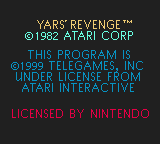
\includegraphics[width=\linewidth]{assets/assets/dmg-ayve/dmg-ayve-7.png}}\end{minipage}\vspace{2pt}
\begin{minipage}{0.45\linewidth}\adjustbox{valign=t}{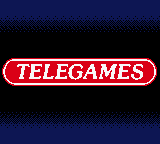
\includegraphics[width=\linewidth]{assets/assets/dmg-ayve/dmg-ayve-8.png}}\end{minipage}\vspace{2pt}
\begin{minipage}{0.45\linewidth}\adjustbox{valign=t}{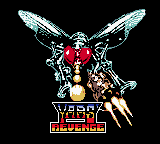
\includegraphics[width=\linewidth]{assets/assets/dmg-ayve/dmg-ayve-9.png}}\end{minipage}\vspace{2pt}
\begin{minipage}{0.45\linewidth}\adjustbox{valign=t}{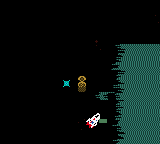
\includegraphics[width=\linewidth]{assets/assets/dmg-ayve/dmg-ayve-10.png}}\end{minipage}\vspace{2pt}
\begin{minipage}{0.45\linewidth}\adjustbox{valign=t}{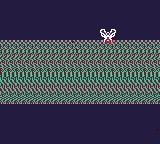
\includegraphics[width=\linewidth]{assets/assets/dmg-ayve/dmg-ayve-11.png}}\end{minipage}
\par\justifying
Those screens are nothing special but the presentation’s brevity has the benefit of making sure you spend all of the game doing one thing: going through the gameplay loop.\par
\FloatBarrier\section*{The Gameplay Loop}
\begin{wrapfigure}{L}{0pt}{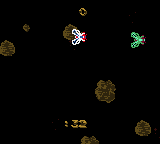
\includegraphics[width=.45\linewidth]{assets/assets/dmg-ayve/dmg-ayve-12.png}}\end{wrapfigure}\noindent
With a game like \emph{Yars’ Revenge}, one thing to keep in mind is that the game is the same short burst of gameplay repeated forever. The only change is a slight enemy speed increase or a difference in the shield of the enemy. The Game Boy version strangely adds the appearance of two new enemies: a kind of blue bullet that freezes you in place if you touch it and a weird squid that brings new shield parts that you can steal before they’re in place. They’re not very interesting, and honestly they start appearing so late in the levels as to not really matter. Their inclusion is puzzling. I had to put in a password to see them because I never played long enough otherwise to get to them.\par
\FloatBarrier\vspace{\baselineskip}\centering
\begin{minipage}{0.45\linewidth}\adjustbox{valign=t}{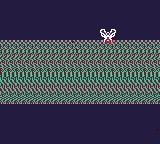
\includegraphics[width=\linewidth]{assets/assets/dmg-ayve/dmg-ayve-13.png}}\end{minipage}\vspace{2pt}
\begin{minipage}{0.45\linewidth}\adjustbox{valign=t}{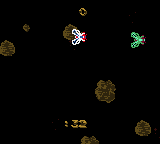
\includegraphics[width=\linewidth]{assets/assets/dmg-ayve/dmg-ayve-14.png}}\end{minipage}
\par\justifying
To break the gameplay loop, the game introduces a weird bonus section. It is reached if you manage to touch a strange shadow of Yar that appears once the Qotile has exploded. It is an obvious attempt to keep the original game’s Easter egg alive. In the original game, if you destroyed the Qotile when it was hurtling towards you as the whirlwind \textbf{and then} you stayed vertical on the same angle as an empty line of the explosion, the initials of Warshaw would flash on the screen. Easter eggs were a trademark of Warshaw, and here the team at Telegames were clearly inspired to keep the easter egg alive with a bonus section.\par
In the bonus section, you have to navigate an asteroid field and stay on top of a \emph{ghost of Yar} to get points. But the asteroids don’t kill you if you touch them, they instead push you back in a jigsaw fashion, just like the Qotile’s orange shield. The whole bonus mini game was obviously an afterthought reusing the physics systems they had already coded for the main game.\par
\FloatBarrier\section*{The Music}
There is no music to speak of. The game features a varying array of digital VCS fart noises. They should have deviated from the original with that one. I guess you should turn the volume off and listen to something else while playing this game. It makes sense; the main character is a fly who keeps buzzing.\par
\FloatBarrier\section*{Conclusion}
\begin{wrapfigure}{R}{0pt}{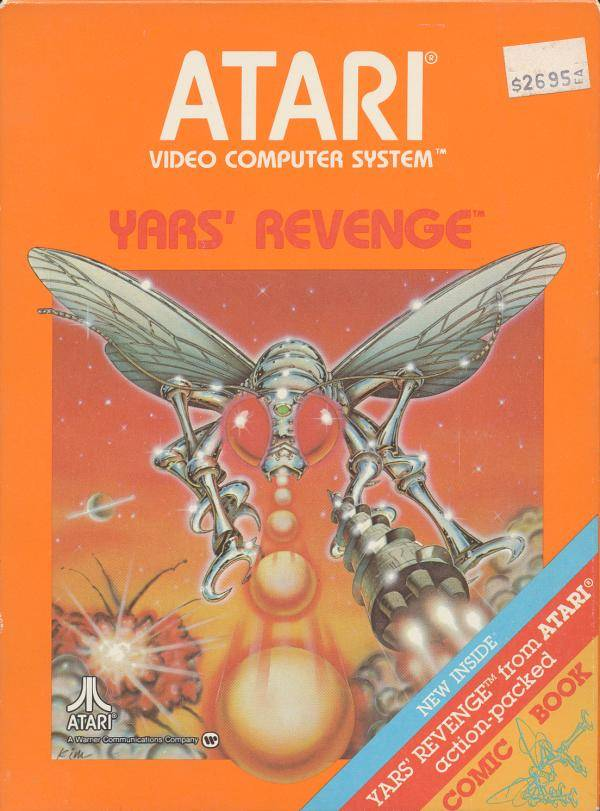
\includegraphics[width=.45\linewidth]{assets/assets/dmg-ayve/dmg-ayve-15.jpg}}\end{wrapfigure}
\emph{Yars’ Revenge} is never on best-of lists because it’s not much to look at and you don’t take it seriously at first glance but it truly is essential in its own weird way. \emph{Yars’ Revenge} is a good example of how to properly adapt a game for the Game Boy. It preserves the feedback loop of the original game, while trying to improve the game in subtle and mostly positive ways. It understands the resolution limitations of the screen and provides tools that allow you to have the proper awareness of things outside that screen. It does suffer from a poor art style: it has anemic pixel art, an absence of music and very weak transition screens. That presentation is amateurish and reeks of a small team left mostly unchecked. However, it’s a good project done adequately by a small team. They put their efforts where it mattered; the gameplay. I’m looking forward to trying their other games, to see if they pulled those projects off. Check Telegames out, their website is still up with a list of all their Game Boy titles!\par
\chapter*{Mega Man: Dr. Wily’s Revenge}\markboth{Mega Man: Dr. Wily’s Revenge}{}\addcontentsline{toc}{chapter}{Mega Man: Dr. Wily’s Revenge}
\vspace{\baselineskip}\begin{figure}[H]{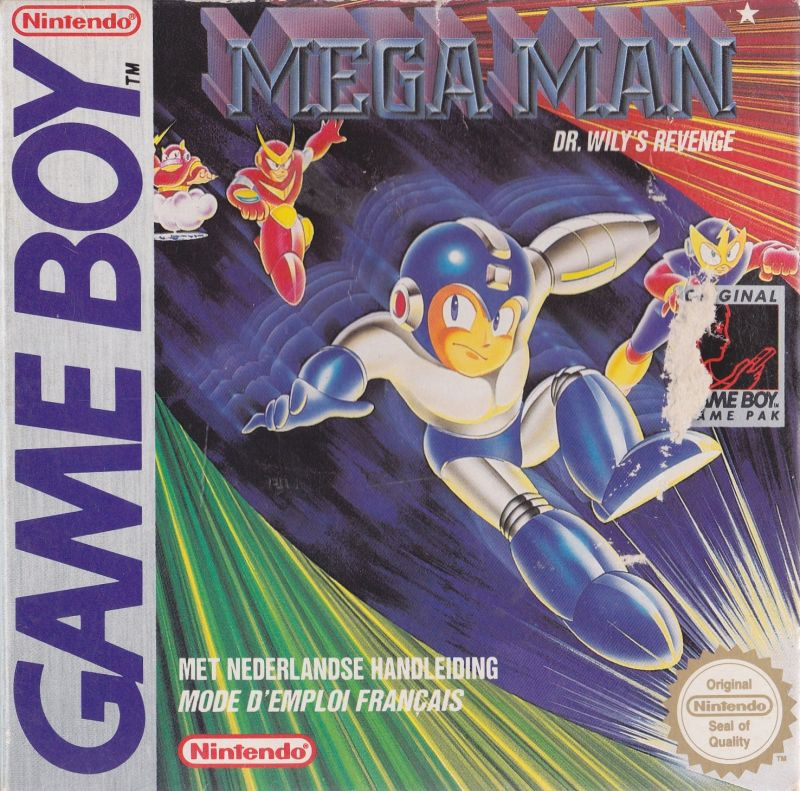
\includegraphics[width=.75\linewidth]{assets/assets/dmg-rw/dmg-rw-1.jpg}}\end{figure}\vspace{\baselineskip}
\begin{itemize}[left=0pt, nosep]
\item Japanese release in July 1991
\item North American release in December 1991
\item European release in 1992
\item Australian release in 1995
\item North American release in May 1996
\begin{itemize}
\item Player’s Choice
\end{itemize}
\item Japanese release in March 2001
\begin{itemize}
\item Nintendo Power
\end{itemize}
\item Developed by Capcom

\end{itemize}
\newpage\FloatBarrier\section*{A First Attempt at the Blue Bomber}
\begin{wrapfigure}{L}{0pt}{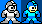
\includegraphics[width=.45\linewidth]{assets/assets/dmg-rw/dmg-rw-2.png}}\end{wrapfigure}\noindent
On Game Boy Essentials, we looked at games no one would include in a best-of list, games that are essential because they’re horrible, but now we get our first game that’s arguably \textbf{unessential}. I had a really hard time deciding whether the first \emph{Mega Man} game on Game Boy was essential or not. Why not consider it? Because it’s too difficult. The jumps required are so precise, the enemy placement so unfair, the bosses’ room so small, that you often find yourself dying because you just couldn’t react properly. I went back and forth on writing an article about it because there are four other classic \emph{Mega Man} games that improved on the formula set in place by this particular title without being as hard. All those are much more essential.\par
Then why do I think it is essential and that you should play it? Because the people at Minakuchi Engineering got the fundamental gameplay exactly right on their first try; they just dropped the ball with everything else. And I think you should play it to witness those two conflicting realities in motion.\par
\FloatBarrier\section*{Minakuchi Engineering}
\begin{wrapfigure}{R}{0pt}{
\includegraphics[width=.45\linewidth]{assets/assets/dmg-rw/dmg-rw-3.png}}\end{wrapfigure}
When you think of who created Mega Man you immediately think of the man people tend to call his father, Keiji Inafune. Inafune is called Mega Man’s father but he seems to have adopted the child during pregnancy. Akira Kitamura created the sprite used for the character and only after that did Inafune come in and create artwork to represent the character on the covers and manuals. Mega Man was built completely backward: a sprite first, a character second. To top it off, Inafune truly became the steward of the \emph{Mega Man} series only starting in 1990 with \emph{Mega Man~3}.\par
Keiji Inafune and the rest of the main \emph{Mega Man} team at Capcom worked on none of the Game Boy titles. \emph{Mega Man: Dr. Wily’s Revenge} is actually the first \emph{Mega Man} game to have been worked on by another studio. Minakuchi Engineering, who got the job, had some experience with the Game Boy. They had previously worked with Nintendo on Game Boy: they co-developed \emph{SolarStriker} with R\&D1.\par
Minakuchi were thus given a daunting task: translate the solid foundations of \emph{Mega Man} for Game Boy.\par
\FloatBarrier\section*{Fundamentals Done Right}
\FloatBarrier\vspace{\baselineskip}\begin{figure}[H]\centering{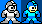
\includegraphics[width=.6\linewidth]{assets/assets/dmg-rw/dmg-rw-4.png}}\caption*{He’s got a new hat!}\end{figure}
What do I mean by fundamentals done right? Look no further than the difference between the NES and Game Boy sprite of Mega Man. Aside from an added black border to his helmet to compensate for the lack of a fifth colour, the Game Boy sprite is pixel-perfect with the NES sprite. I have seen one other slight change; they moved his arms further up when he jumps making him use less horizontal space when in the air.\par
\FloatBarrier\vspace{\baselineskip}\begin{figure}[H]\centering{\includegraphics[width=.6\linewidth]{assets/assets/dmg-rw/dmg-rw-5.png}}\caption*{Game Boy Mega Man overlaid over NES sprite. Look at the arms.}\end{figure}
Considering that Capcom never once altered the sprite of Mega Man for six games on NES, I’m sure they were the ones who decided on so few sprite changes for the Game Boy. To me it’s so funny that the sprite in the games was always sacrosanct but the box art was consistently \emph{all over the place}. You have frumpy redrawn faces for American audiences, separate redrawn faces for European audiences, weird gun arms, wrong colours, broken proportions, the works. Anyway, I would bet Capcom designers drew the Game Boy sprites internally at Capcom and then handed them to Minakuchi. Knowing that the sprite was designed first, this seems a likely explanation. This decision not to redraw Mega Man to be any smaller means that Mega Man covers a much larger percentage of the screen than on NES. See for yourself.\par
\FloatBarrier\vspace{\baselineskip}\begin{figure}[H]\centering{\includegraphics[width=.6\linewidth]{assets/assets/dmg-rw/dmg-rw-6.png}}\caption*{A screenshot of \emph{Mega Man I} on Game Boy overlaid over \emph{Mega Man~1} on NES. See how much more of the level you can see on NES.}\end{figure}
You can see here how much you \textbf{can’t} see on Game Boy. Something had to give. There are other games like \emph{Super Mario Land} or the first \emph{Batman} game on Game Boy that took different approaches to the limited screen of the system. \emph{Mega Man} on Game Boy’s approach: don’t change the Blue Bomber, change the world around him. There were games with large sprites before \emph{Mega Man}. \emph{Fist of the North Star}, \emph{TMNT: Fall of the Foot Clan}, \emph{Ninja Boy}, \emph{Metroid~II: Return of Samus}, and many more. But while most games released before then were not always successful at their attempt to use large-sized sprites on Game Boy, \emph{Mega Man} did something really right. This first \emph{Mega Man} title will perfect the standard way of making a NES game work on Game Boy: you adapt every element of the gameplay for the smaller screen without changing the size of the characters and enemies.\par
The first thing they had to change was the size of the environment. Mega Man controls the same and looks the same so he jumps a full third of the screen on Game Boy. This comes with a lot of caveats. They could not for example put a pit with a flying enemy heading your way from the other side of the screen. If this were to happen the enemy would appear too quickly, you would have no time to react and end up at the bottom of the pit a very frustrated player. All sorts of little details had to change to keep the experience fun.\par
\FloatBarrier\vspace{\baselineskip}\begin{figure}[H]\centering{\includegraphics[width=4.85cm]{assets/assets/dmg-rw/dmg-rw-7.png}}\caption*{Something as innocuous as an enemy falling from the top of the screen had to be reengineered when done on Game Boy.}\end{figure}
\FloatBarrier\section*{Lack of Practice}
They did succeed in making sure the upcoming environmental challenges were always on the screen. Unfortunately, they made \textbf{way} too many jumps too difficult to clear when adjusting the gameplay. Pits in this game are always painful and difficult. Some of them seem to give you only a couple pixels of leeway.\par
The enemies are usually the same size and act the same as on NES, and are as varied. It’s great for presentation but that means they give you less time to react since they’re always so big and so close to you. Imagine a robot with a shield in front of you; when he shoots you have less time to jump than you would on NES.\par
\FloatBarrier\vspace{\baselineskip}\centering
\begin{minipage}{0.45\linewidth}\adjustbox{valign=t}{\includegraphics[width=\linewidth]{assets/assets/dmg-rw/dmg-rw-8.png}}\end{minipage}\vspace{2pt}
\begin{minipage}{0.45\linewidth}\adjustbox{valign=t}{\includegraphics[width=\linewidth]{assets/assets/dmg-rw/dmg-rw-9.png}}\end{minipage}
\par\justifying
Big enemies are even more of a pain to deal with. Those encounters were not made for the small Game Boy but they still tried to make them happen. You would encounter those big enemies in all kinds of varied situations on NES but here they had to relegate them to enclosed spaces. Coupled with the fact that all the rooms have walls and floors that are very thick, those encounters feel cramped and unpleasant. Even if they did redraw those large enemies to be smaller. The bosses suffer from the same thick walls problem. For \emph{Mega Man IV}, they would make the walls as thin as they could, giving you just a bit more space to fight the master robots. We’re talking a dozen pixels but the effect is striking. In \emph{Mega Man I}, you feel the cramped screen. In \emph{Mega Man IV}, the boss rooms feel big enough.\par
\begin{wrapfigure}{L}{0pt}{\includegraphics[width=.45\linewidth]{assets/assets/dmg-rw/dmg-rw-10.png}}\end{wrapfigure}\noindent
Did you know that \emph{Mega Man I} on Game Boy also has four robot Masters from \emph{Mega Man~2} on NES? It’s a kind of ad hoc tradition with the Game Boy titles to include four robot masters from the numbered NES counterpart and four from the next game. Here the tradition was born, and once you reach the teleporters in the last Wily stage where you would usually refight the robot masters, you get a surprise! Flash Man, Quick Man, Bubble Man, and Heat Man from \emph{Mega Man~II} are who you face instead. The game did not include Guts Man and Bomb Man from \emph{Mega Man~1}, but the four extra bosses are meant to be a twist on the formula; unfortunately it kind of falls flat. They appear so late in the game that their presence feels like an afterthought. There’s no buildup, no expectations, they just suddenly appear. With each new \emph{Mega Man} game the four extra robot masters would start appearing earlier and earlier and gain in prominence.\par
Finally, the password system is exactly the same as on NES, which does not translate well to a portable system. You get a different password after every completed robot master, which is nice and feels appropriate but once you hit the Wily stages, you get one password to start from the first stage and that’s it. I’ve always felt the lack of Wily passwords was a shame on NES. On Game Boy, where you play much shorter play sessions, it’s downright exasperating.\par
\FloatBarrier\section*{The Things Unsaid}
\begin{wrapfigure}{R}{0pt}{\includegraphics[width=.45\linewidth]{assets/assets/dmg-rw/dmg-rw-11.png}}\end{wrapfigure}
I could talk about the many other things related to the game: the level design inspired by the first game, the music, how the presentation makes the background elements non-obstructive, the gameplay loops, the ending, whatever. I’m not going to dwell on those things, however, because they’re not what makes this game essential. They’re kind of inconsequential. I’ve already talked about what makes \emph{Mega Man: Dr. Wily’s Revenge} essential. The rest is serviceable, evocative of a \emph{Mega Man} game but clearly on the cheap side.\par
\FloatBarrier\section*{Conclusion}
Ultimately, I think Capcom knew they had good fundamentals but a flawed product with \emph{Mega Man: Dr. Wily’s Revenge}. Why? They gave the job of making \emph{Mega Man~II} on Game Boy to a different developer, Biox. They ended up releasing \emph{Mega Man~II} in Japan a mere five months after the first game. To me that screams of “we know the first one was too hard but this second one’s easier.” However, \emph{Mega Man~II} was too easy and kind of crappy, so Capcom \textbf{went back to Minakuchi Engineering for all the following Game Boy Mega Man games}. That’s why this game is essential. It’s a testament to Capcom’s trust that this group of developers did a great job setting up the fundamentals of \emph{Mega Man} with the first game and were trusted with getting the franchise back on track when Biox led it askew. They ultimately did. We’ll get to those better games in due time.\par
\chapter*{Super Mario Land}\markboth{Super Mario Land}{}\addcontentsline{toc}{chapter}{Super Mario Land}
\vspace{\baselineskip}\begin{figure}[H]{\includegraphics[width=.75\linewidth]{assets/assets/dmg-ml/dmg-ml-1.jpg}}\end{figure}\vspace{\baselineskip}
\begin{itemize}[left=0pt, nosep]
\item Japanese release in April 1989
\item North American release in July 1989
\item European release in September 1990
\item European release in 1990
\item Australian release in 1990
\item Asian release in 1990
\item Brazilian release in 1993
\item North American release in May 1996
\begin{itemize}
\item Player’s Choice
\end{itemize}
\item European release in 1996
\begin{itemize}
\item Game Boy Nintendo Classics
\end{itemize}
\item North American release in November 1999
\begin{itemize}
\item 1999 Player’s Choice
\end{itemize}
\item Japanese release in March 2000
\begin{itemize}
\item Nintendo Power
\end{itemize}
\item Developed by Nintendo

\end{itemize}
\newpage\FloatBarrier\section*{2-Bit Mario}
\begin{wrapfigure}{L}{0pt}{\includegraphics[width=.45\linewidth]{assets/assets/dmg-ml/dmg-ml-2.png}}\end{wrapfigure}\noindent
\emph{Super Mario Land} is a technological dead end with its roots in the Game \& Watch portables of the 80s. Featuring design decisions that were abandoned by almost all Game Boy developers, \emph{Super Mario Land} is nonetheless essential because it is the first game ever made for Game Boy.\par
Made by Gunpei Yokoi and his team at R\&D1, without \emph{Super Mario Land} there simply is no Game Boy. The game was meant to prove that you could have platform games be as fun as what Nintendo was doing on NES. On that front it succeeded but it’s also an interesting example of a strategic pivot by Nintendo. Once they discovered \emph{Tetris}, Nintendo sidelined this Mario game and bet heavily that the Game Boy and \emph{Tetris} were a better story to sell to potential players. Their proof-of-concept \emph{Mario} game could not sell the Game Boy to as many people as the falling blocks of \emph{Tetris}. Of course, they released this game and marketed it heavily but in markets where they advertised and sold bundles on release the Game Boy came with \emph{Tetris}, not \emph{Super Mario Land}. Nintendo worked hard to equate Game Boy with \emph{Tetris}. Working from Tetris’ success as this vanguard from the system, Game Boy developers knew what to copy when they made puzzle games. Platform games on Game Boy had to pave another path to success; \emph{Super Mario Land’s} ideas were not easily marketable.\par
\FloatBarrier\section*{A Tiny Slice of History}
Research \& Development~1, Yokoi’s division within Nintendo, was riding high at the end of the 80s. The Game \& Watch portable first introduced in 1980 were still successful in 1989. Using the popularity of the new franchises created by Shigeru Miyamoto for the Famicom, Multi Screen games like \emph{Zelda} featured maps, items, progression, continues, even bosses.\par
\FloatBarrier\vspace{\baselineskip}\begin{figure}[H]\centering{\includegraphics[width=.75\linewidth]{assets/assets/dmg-ml/dmg-ml-3.png}}\caption*{The \emph{Zelda} Game \& Watch}\end{figure}
They basically tried everything they could to make the Game \& Watch games feel as expansive as they could, recreating the best Nintendo games of the Famicom and NES on tiny tailor-made calculator screens. At this point I kind of have to explain what the Game \& Watch titles were. Game \& Watch games used black and white LCD screens with pre-defined LCD graphics permanently imprinted on the screen. Just like a calculator can only display little shapes that add up to show numbers the Game \& Watch used the same screen technology but with intricately drawn characters. Those discrete elements cannot move around the screen just like the characters on a calculator display can’t start jumping around. This means you have to be very inventive with your game design to imply movement and action. Add to that silkscreened overlays for background elements and you have dedicated portable systems with loads of charm and the ability to display a clock (hence the title Game \& Watch). Those little portables were more toys than video games, however, obviously limited to one game per little machine. Many companies ultimately copied Nintendo’s design, making the LCD single game concept pioneered by Nintendo synonymous with portable gaming in the 80s. However, Nintendo saw a terrible future for the Game \& Watch family. A black cloud was hanging over the market of single-game LCD portables.\par
\FloatBarrier\vspace{\baselineskip}\begin{figure}[H]\centering{\includegraphics[width=.5\linewidth]{assets/assets/dmg-ml/dmg-ml-4.jpg}}\end{figure}
\FloatBarrier\section*{Sidenote}
When Nintendo abandoned the Game \& Watch concept in 1991 Tiger Electronics was by then the king of the LCD games. Starting in 1988, they had managed to reduce production costs to oblivion and had flooded the market with crappy licensed games of everything under the sun. In time, this included old franchises like \emph{The Flintstones}, popular movies like \emph{Batman Returns} and \emph{Jurassic Park}, blockbuster arcade titles like \emph{Street Fighter~II} or \emph{Mortal Kombat} and corny 80s sitcoms like \emph{Full House}. I kid you not there even was a \emph{MC Hammer} LCD game. As someone born in 1986, I never laid hands on a Game \& Watch but by the middle of the 90s I can attest that Tiger Electronics games were everywhere.\par
\FloatBarrier\vspace{\baselineskip}\centering
\begin{minipage}{0.45\linewidth}\adjustbox{valign=t}{\includegraphics[width=\linewidth]{assets/assets/dmg-ml/dmg-ml-5.jpg}}\end{minipage}\vspace{2pt}
\begin{minipage}{0.45\linewidth}\adjustbox{valign=t}{\includegraphics[width=\linewidth]{assets/assets/dmg-ml/dmg-ml-6.jpg}}\end{minipage}
\par\justifying
The larger ones were cheap, the smaller ones came with other toys and I even remember getting a Tiger Electronics watch of the \emph{Pagemaster} movie in a cereal box! They all had one point in common though: they were \textbf{terrible} games with brain-dead gameplay. By then Nintendo had wisely moved on. If like me you have only played the Tiger Electronics LCD games, try a Nintendo Game \& Watch title. They’re on a completely different order of magnitude. A great way to play them is with the \emph{Game \& Watch} games on Game Boy. That’s how I first discovered them.\par
\FloatBarrier\section*{Dot Matrix Gameplay}
Back in the 80s Yokoi and the people at R\&D1 were putting a lot of efforts into their LCD games (it showed) but they were probably itching for a richer experience, desiring to allow their customers to play games as complex as the Famicom titles that Miyamoto’s team at R\&D4 were making (R\&D4 was renamed Entertainment Analysis \& Development [EAD] in 1989, as all of this was happening). R\&D1 was originally tasked with creating Nintendo’s arcade titles but when that fizzled away, R\&D1 pivoted hard to the Game \& Watch titles. When the time came to move ahead with a new concept, Yokoi’s strategy came in handy. He was always trying to find new ways to use seasoned technology; he described it as \emph{Lateral Thinking of Withered Technology}. What does that mean? Using cheap, simple technologies that you know very well in interesting ways. Developments in the early 80s, which fit in that exact mindset, allowed for inexpensive low-power monochrome pixel displays called super-twisted nematic LCDs. Those displays had very interesting qualities over standard TFT LCDs (TFT LCDs are what you would find in the Game Gear, the Atari Lynx and laptops of the time). This all fell in line with Yokoi’s hardware strategy; STN LCDs were cheap to produce, very energy-efficient compared to TFT LCDs, and they used pixels instead of the discrete crystals of the Game \& Watch. This is why the Game Boy proudly proclaimed itself a Dot Matrix with Stereo Sound above the screen: R\&D1 is saying they’re proud because its screen is made with pixels. This meant that you could display anything you could program. The fact that the screen ended up pea-soup green, monochrome and with very pronounced ghosting were all side effects Yokoi was ultimately willing to live with in exchange for great battery life and an affordable cost.\par
Slap a weird mix between a Z80 and an Intel~8080 made by Sharp in there (another cheap technology that was very well understood in the 80s), add the controls of the NES (Yokoi had previously invented the D-pad with the Game \& Watch) and you’re all set. Surprisingly, recent interviews with Satoru Okada, who worked directly under Gunpei Yokoi have shown that the main man was not necessarily on board with the idea of the Game Boy as a portable NES. Okada claims that Yokoi instead wanted something cheaper and more similar to the Game \& Watch line, a better MB Microvision in a sense. Okada basically built the Game Boy without Yokoi’s direct involvement. You could argue that to convince the naysayers, R\&D1 needed a proof-of-concept; a way to show people what their new thing was capable of. For the Game Boy, that was \emph{Super Mario Land}.\par
\FloatBarrier\section*{Sarasaland}
We’ve talked extensively about the history that led to \emph{Super Mario Land}, but how does the game play? The first thing to keep in mind is that no other game is quite like it. While the overwhelming majority of platform games on Game Boy features sprites who have the same pixel count as their NES counterparts, \emph{Super Mario Land} chose to use a proportional perspective.\par
\FloatBarrier\vspace{\baselineskip}\begin{figure}[H]\centering{\includegraphics[width=.6\linewidth]{assets/assets/dmg-ml/dmg-ml-7.png}}\caption*{\emph{Super Mario Land} superimposed over \emph{Super Mario Bros.} You can see how the space ahead of Mario is very similar.}\end{figure}
Both \emph{Super Mario Bros.} and \emph{Super Mario Land} share the same overall proportions on the screen. Even though one is on a standard NTSC TV screen with a generous resolution and the other is on the limited Game Boy screen Mario has the same amount of ground in front of him in both games. To achieve such a large field of play on Game Boy the sprites are ultimately minuscule. If you compare the sprites of Mario \& Wario on all of their Game Boy games you will understand what I mean by minuscule. The only other game I know that uses sprites this small for a platform game is \emph{Batman: The Video Game}. If you know any other one with similar proportions on Game Boy, let me know!\par
\FloatBarrier\vspace{\baselineskip}\begin{figure}[H]\centering{\includegraphics[width=.6\linewidth]{assets/assets/dmg-ml/dmg-ml-8.png}}\caption*{Sprites from all the \emph{Mario} \& \emph{Wario} games on Game Boy. Mario’s head in \emph{Super Mario Land} is smaller than Wario’s butt!}\end{figure}
That initial decision to keep the same overall proportions as on NES means the gameplay is unique. The scenery runs by very fast compared to other games on Game Boy and the jumps are enormous. The screen never scrolls up or down; the only direction the screen ever goes is right, just like \emph{Super Mario Bros.} on NES. With so large a play field there is a truly rare sight on Game Boy; levels have distinct upper and lower passages on the same level without any upward or downward scrolling.\par
\FloatBarrier\vspace{\baselineskip}\begin{figure}[H]\centering{\includegraphics[width=4.85cm]{assets/assets/dmg-ml/dmg-ml-9.png}}\caption*{You can go above or under without any vertical scrolling. Unbelievable, but this is absurdly rare on Game Boy.}\end{figure}
\begin{wrapfigure}{L}{0pt}{\includegraphics[width=.45\linewidth]{assets/assets/dmg-ml/dmg-ml-10.png}}\end{wrapfigure}\noindent
\emph{Super Mario Land}, as we’ve established, came out of a studio that was used to making Game \& Watch games. It shows. The most potent examples to me are the weird walking UFO enemies in the second world. They’re made of two distinct separate parts. When you jump on the enemy it loses its top part and keeps milling about with its bottom part. Since neither part touch, you would not be mistaken to think this hamburger of an enemy would be made of two LCD crystals like on a Game \& Watch.\par
This, to me, is the most potent example of something clear with \emph{Super Mario Land}: it was built by a team renown for their Game \& Watch games. The way the turtle shells explode when hit, the backgrounds, the way enemies lose non-overlapping parts of their body when you first hit them. I can’t find any information that the two designers, Hirofumi Matsuoka and Masahiko Mashimo, were Game \& Watch designers but it sure does look like \emph{Super Mario Land’s} graphic designers kind of forgot they could have overlapping and interlocking elements.\par
\FloatBarrier\section*{SMB for DMG}
Since the game is so clearly meant to emulate \emph{Super Mario Bros.} how does it compare? Not that favourably to be honest. Mario does not control as well as on NES, having short momentum and limited control on diagonal jumps. This is the game’s biggest sin; usually when one thinks of a \emph{Mario} game one thinks of flawless controls. This is not the case here. They’re not perfect and it hurts the game’s enjoyment. On the other hand, the checkpoints are generous and the game is not stingy on the extra lives. The game is not frustrating. I’d say it’s much easier than \emph{Super Mario Bros.} .\par
\FloatBarrier\section*{Levels and Length}
\emph{Super Mario Land} did one thing that everybody immediately copied: its length. It codified how long a game on Game Boy should be with its twelve levels instead of the thirty-two of \emph{Super Mario Bros.} on NES. Ultimately you get around a third the content as \emph{Super Mario Bros.} and a lot of Game Boy games will follow that general rule that it first established. It will take years to start finding original games that are as long as console games on Game Boy.\par
\FloatBarrier\vspace{\baselineskip}\begin{figure}[H]\centering{\includegraphics[width=.6\linewidth]{assets/assets/dmg-ml/dmg-ml-11.png}}\caption*{\emph{Super Mario Land} features two shooter levels. The last level, with the last boss, is even one of them. They’re nothing to write home about.}\end{figure}
The levels are also not as interesting and memorable as on NES. Even though the building blocks are more varied and the enemies truly weird the levels are sparsely populated (they were probably very careful with enemy placement due to the poor screen) and the obstacles are not that inspired. Interestingly, the game separates its twelve levels in four distinct worlds with very clear real-world analogues.\par
\FloatBarrier\vspace{\baselineskip}\centering
\begin{minipage}{0.45\linewidth}\adjustbox{valign=t}{\includegraphics[width=\linewidth]{assets/assets/dmg-ml/dmg-ml-12.png}}\captionsetup{labelformat=empty}\captionof{figure}{Egypt}\end{minipage}\vspace{2pt}
\begin{minipage}{0.45\linewidth}\adjustbox{valign=t}{\includegraphics[width=\linewidth]{assets/assets/dmg-ml/dmg-ml-13.png}}\captionsetup{labelformat=empty}\captionof{figure}{The Bermuda Triangle}\end{minipage}\vspace{2pt}
\begin{minipage}{0.45\linewidth}\adjustbox{valign=t}{\includegraphics[width=\linewidth]{assets/assets/dmg-ml/dmg-ml-14.png}}\captionsetup{labelformat=empty}\captionof{figure}{Easter island}\end{minipage}\vspace{2pt}
\begin{minipage}{0.45\linewidth}\adjustbox{valign=t}{\includegraphics[width=\linewidth]{assets/assets/dmg-ml/dmg-ml-15.png}}\captionsetup{labelformat=empty}\captionof{figure}{China}\end{minipage}
\par\justifying
This is another aspect of Mario that is not traditional. When one thinks of the setting of Mario games you think of blocks, tunnels, castles, anything \emph{but} adaptations of real-world locations. \emph{Super Mario Bros. 3} is all Piranha plants and pipes, not anything realistic. I mean there are pyramids but they don’t have any Egyptian hieroglyphs or mummies. The exception to the rule is \emph{Super Mario Bros. 2} with its very clear Arabian influence but that was originally another game based on a Japanese festival that was influenced by \emph{One Thousand and One Nights}. I’ve read rumours that \emph{Super Mario Land} was originally not a \emph{Mario} game and got turned into one during development. All its off-key weird levels including the side-scrolling shooter levels might make you think that. Seriously, who thought of dumping Mario in a submarine? A prop plane? Why does Mario start World~2 coming out of a flying saucer? Whatever the case may be, the most important thing to keep in mind is \emph{Super Mario Land} was not made by Mario’s father, Miyamoto and his team, but by Yokoi’s team. To me that’s enough explanation for why the controls and the levels are weird. Everything about this game is off-key. It’s a cavalcade of weird enemies and bosses.\par
\FloatBarrier\vspace{\baselineskip}\centering
\begin{minipage}{0.45\linewidth}\adjustbox{valign=t}{\includegraphics[width=\linewidth]{assets/assets/dmg-ml/dmg-ml-16.png}}\end{minipage}\vspace{2pt}
\begin{minipage}{0.45\linewidth}\adjustbox{valign=t}{\includegraphics[width=\linewidth]{assets/assets/dmg-ml/dmg-ml-17.png}}\end{minipage}\vspace{2pt}
\begin{minipage}{0.45\linewidth}\adjustbox{valign=t}{\includegraphics[width=\linewidth]{assets/assets/dmg-ml/dmg-ml-18.png}}\end{minipage}\vspace{2pt}
\begin{minipage}{0.45\linewidth}\adjustbox{valign=t}{\includegraphics[width=\linewidth]{assets/assets/dmg-ml/dmg-ml-19.png}}\end{minipage}\vspace{2pt}
\begin{minipage}{0.45\linewidth}\adjustbox{valign=t}{\includegraphics[width=\linewidth]{assets/assets/dmg-ml/dmg-ml-20.png}}\end{minipage}\vspace{2pt}
\begin{minipage}{0.45\linewidth}\adjustbox{valign=t}{\includegraphics[width=\linewidth]{assets/assets/dmg-ml/dmg-ml-21.png}}\end{minipage}\vspace{2pt}
\begin{minipage}{0.45\linewidth}\adjustbox{valign=t}{\includegraphics[width=\linewidth]{assets/assets/dmg-ml/dmg-ml-22.png}}\end{minipage}\vspace{2pt}
\begin{minipage}{0.45\linewidth}\adjustbox{valign=t}{\includegraphics[width=\linewidth]{assets/assets/dmg-ml/dmg-ml-23.png}}\end{minipage}\vspace{2pt}
\begin{minipage}{0.45\linewidth}\adjustbox{valign=t}{\includegraphics[width=\linewidth]{assets/assets/dmg-ml/dmg-ml-24.png}}\end{minipage}
\par\justifying
But it’s all off-key in \emph{hindsight}. \emph{Mario} games are a \textbf{very} codified franchise now but that wasn’t the case back in 1989 when this game was made and released. So that’s why it’s so essential. It’s a weird side step in one of video game’s most codified franchise made without Miyamoto’s involvement. Back when the Game Boy was released it was just a fun portable \emph{Super Mario Bros.} derivative, a kind of throwback to 1986 NES. Nobody took it to task for its off-brand sentiment, since \emph{Super Mario Bros. 2} had expanded the scope of what a Mario game was. In Japan they had \emph{Super Mario Bros. 3} when the Game Boy was released, which I’m sure helped to show \emph{Super Mario Land} for what it truly was: a throwback to a simpler time.\par
\FloatBarrier\section*{Hip Tanaka Shoots and Scores}
Hip Tanaka, Nintendo’s legendary music composer, is very good at knowing exactly what kind of music a game needs and \emph{Super Mario Land} is testament to that. He’s given the task of making music for a portable analogue to Koji Kondo’s \emph{Super Mario Bros.} soundtrack and he does exactly that. The whole soundtrack is as memorable as \emph{Super Mario Bros.} It’s unequivocally \emph{Mario}.\par
In a rare case of musical borrowing, the star power-up music is a rendition of a classic composition, Offenbach’s \emph{Infernal Gallop}. You know, cancan music. Another off-key thing about this game. Tanaka never again lifted classical music wholesale for a project. But why do it here? I presume that the Game Boy’s limited colour palette prevented the cycling of colours you see at the end of a Starman sequence on NES. Thus, something else was needed to indicate the end of a Starman; you don’t want to get hit because you didn’t realize it was nearly over. So Hip Tanaka probably went with the first little musical ditty he could think of that everyone knew by heart. That way, everyone would know when the power-up is over, because we all instinctively know the length of this short musical segment. Very ingenious.\par
\FloatBarrier\section*{Conclusion}
\emph{Super Mario Land} is a \emph{Mario} game but not one coming from Nintendo’s wunderkind designer Shigeru Miyamoto; instead it’s from Nintendo’s genius toy inventor Gunpei Yokoi, and it shows. The game has weird mechanics, a peculiar atmosphere and includes two horizontal shooter levels. It’s off brand \emph{Mario}. It ultimately shows the differences in philosophy between both teams. On the one hand, R\&D1 who built the Game Boy, and on the other EAD, Miyamoto’s team that was Mario’s home. R\&D1 was clearly more comfortable with hardware and their own concepts like Metroid and Kid Icarus. They gave Mario a fair shake but ultimately did not capture the lighting in a bottle of \emph{Super Mario Bros. *. For all this, *Super Mario Land} is truly unique.\par
\chapter*{Final Fantasy Adventure}\markboth{Final Fantasy Adventure}{}\addcontentsline{toc}{chapter}{Final Fantasy Adventure}
\vspace{\baselineskip}\begin{figure}[H]{\includegraphics[width=.75\linewidth]{assets/assets/dmg-ff/dmg-ff-1.jpg}}\end{figure}\vspace{\baselineskip}
\begin{itemize}[left=0pt, nosep]
\item Japanese release in June 1991
\item North American release in November 1991
\item European release in 1993
\item North American release in 1998
\begin{itemize}
\item Reprint
\end{itemize}
\item Developed by SquareSoft

\end{itemize}
\newpage\FloatBarrier\section*{Mana without the Mania}
\begin{wrapfigure}{L}{0pt}{\includegraphics[width=.45\linewidth]{assets/assets/dmg-ff/dmg-ff-2.png}}\end{wrapfigure}\noindent
\emph{Final Fantasy Adventure} is unique. It’s a gaiden title of \emph{Final Fantasy} that subsequently transformed into its own franchise. Some of it is awesome. Some of it is weird. Some of it is bad. But ultimately you’ll have fun with \emph{Final Fantasy Adventure}. That’s why it’s essential.\par
\FloatBarrier\section*{Memo about Screenshots}
I play games for Game Boy Essentials on my trusty backlit Game Boy Advance SP and then I go and gather screenshots on an emulator. This means that to have screenshots of the game I need to play through everything twice. \emph{Final Fantasy Adventure} being a bit too long for me to play twice, this article will thus be light on screenshots. If you want to see pictures of the game, I recommend looking up lparchive.org, who have a Let’s Play from the Something Awful forums. Interestingly, the \emph{modern} definition of a Let’s Play is a commented video of a play-through of a game. It originally meant a written post with pictures commenting a typical play-through of a game. Look it up.\par
\FloatBarrier\section*{Prints and Reprints}
Let’s talk a bit about history. A long time ago, in January 1997, Squaresoft released \emph{Final Fantasy~VII} on PlayStation in North America and everyone went \textbf{bonkers}. “You mean the game is in 3D! With videos! It’s like real life!”\par
It had everything: Giant swords, cyberpunk aesthetics, casual racism, amnesia!\par
\begin{wrapfigure}{R}{0pt}{\includegraphics[width=.45\linewidth]{assets/assets/dmg-ff/dmg-ff-3.jpg}}\end{wrapfigure}
To capitalize on this newfound craziness for all things \emph{Final Fantasy}, Sunsoft struck a unique deal with SquareSoft. You see, between 1989 and 1991 SquareSoft had released four under-appreciated games on Game Boy. They were \emph{SaGa} and \emph{Seiken Densetsu} games. However, when they brought them to North America between 1990 and 1993 SquareSoft decided to call them \emph{Final Fantasy Legend I}, \emph{II} \& \emph{III} and \emph{Final Fantasy Adventure}; they probably hoped to capitalize on the burgeoning popularity of the series in North America. SquareSoft’s attempt to bring the RPG to Game Boy was kind of forgotten by 1998, when \emph{Final Fantasy~VII} transformed the series from the best-known franchise of a niche genre to the \textbf{most important game of all time, oh my god Cloud is so badass guys!} For SquareSoft and Sunsoft, it was too good to be true. Four games with the title of the hot fad of 1998 that were pretty much ignored back when originally released. Sunsoft jumped on the opportunity, signed a deal with SquareSoft and reprinted those old games for Game Boy in 1998. Their timing was perfect: they rereleased the four games just six months before the Game Boy Color came out. That meant they did not have to deal with an audience that would have expected Color support for those old titles.\par
But \textbf{why} where they kind of ignored back when originally released? Because RPGs were not exactly the most popular thing in 1991 and the Game Boy back then was mostly seen as a puzzle machine. Longish Japanese role-playing games with crazy levelling systems were not meant for mainstream Game Boy appeal. The gaming world was very different after \emph{Final Fantasy~VII}. Here’s a taste of that world.\par
I was only twelve in 1998 when I encountered those four reprinted games in a Wal-Mart. They were all there in a row in a game display case. To my twelve-year-old self, this was a glorious sight. I had already seen \emph{Final Fantasy~VI}, a friend had rented this amazing game called \emph{Chrono Trigger} for his birthday, older friends had shown me \emph{Final Fantasy~VII} on their PlayStation (I had wisely chosen to ask my parents for a Nintendo~64) and I think I might have played \emph{Final Fantasy IV} on ZSNES back then. I’m a bit foggy on the exact dates of my descent into piracy, but I do vividly remember making a school video presentation about NESticle in the 8th grade in 1999. I am that big of a nerd. Anyway, I was riding the \emph{Final Fantasy} hype train \textbf{hard}. Before me stood not one but \textbf{four} Game Boy \emph{Final Fantasy} games. I somehow managed to persuade my mother to buy me one game. I then had to choose. Being a crazy completionist, I chose \emph{The Final Fantasy Legend}, to start with the first game. I got \emph{Final Fantasy Adventure} later on, when I saw it in another store. Don’t worry, we’ll get to the other Game Boy \emph{Final Fantasy} games in due time. Today though, \emph{Final Fantasy Adventure} gets to shine.\par
\FloatBarrier\section*{Description}
\emph{Final Fantasy Adventure} can be summarized very succinctly: A linear \emph{Legend of Zelda} knockoff with RPG elements. Let’s now unpack that description in way too many words.\par
\FloatBarrier\section*{Linear}
\emph{Final Fantasy Adventure} may first lead you to believe it uses an open world map like a \emph{Legend of Zelda} but it doesn’t. The game instead has a story-driven path that you must follow. You start off around the middle of the world map, and you go through all the sections of the game as the story dictates. It’s not a disadvantage \emph{per se}. It’s fun to follow along the path of the game, playing through the flimsy dumb 90s RPG attempt at a story. While you can at one point go back to all the previous sections of the game, this is useless. In a game with a truly open world you go back to places you’ve been before to unearth secrets. Here, there are no secrets to be found in completed sections and enemies are a pest: they hurt for literally 1 damage and the experience points they give are so meagre it might as well be nothing. The only thing that will come out of you exploring the map is you’ll get lost in old sections of the game and you’ll eventually forget where you were supposed to go.\par
The openness of the game is actually a masterclass in what not to do when you want a cohesive world map. The geography of the world is all weird. The map is one incomprehensible continent with no real sense of place and sinewy rivers that make no sense. Deserts are right next to ice plains; every region of the game is next to another with no logic behind their placement. To top it off, when you can access it all at once, you navigate it with a robotic chocobo that can run on water but can’t fly, so you get stuck on every nook and cranny without having an easy way to go from one place to the next. To me the best example of good map design is how they deal with the sides of the map. In any SquareSoft game with a world map, say \emph{Final Fantasy V} for example, you have a large body of water between the sides of the rectangular map to help you make sense of where you are. That way you’re confused just enough to buy into the fiction that you’re on a spherical world. In this game, you’re all the way to the right of the map and go one screen right and suddenly you’re all the way to the left without a screen of water to kind of transition you from one side of the world to the other. I vividly remember trying to make sense of the geopolitical atmosphere of the \emph{Final Fantasy IV} world when I was a kid. I never did it with this game.\par
\FloatBarrier\section*{Legend of Zelda Knock-Off}
Ishii Kōichi, father of the Chocobo, co-composer of the Crystal Theme and developer at SquareSoft looked at \emph{The Legend of Zelda} and said: \emph{I want to do something like \textbf{that}.} He tried to get such a game made for years and he finally got it done on Game Boy, when SquareSoft management finally gave him the go ahead to make an action game on Game Boy. So there’s no surprise the game is so similar to \emph{Zelda}.\par
The game features the same grid-based movement as the first \emph{Zelda} game. You get the same overall way to move, the same overall way to attack and the exact same screen to screen scrolling of \emph{The Legend of Zelda}. To me that’s cool because that gameplay system has not been used often enough by good developers. At the time \emph{Final Fantasy Adventure} came out, games that emulated \emph{The Legend of Zelda} were hit or miss. I’m not a developer, but I guess it’s very easy to mess up an action-adventure game. Which leads me to a point they did mess up: the enemies.\par
The movement patterns of enemies is uninspired. They jump all around the screen with a complete disregard for the obstacles on the map and they don’t react to being hit by you or ever try to actively attack you. You don’t feel like the enemies are meaningful, they’re just there. In contrast, \emph{Zelda} enemies obey the same rules as Link. Some enemies can jump above walls and obstacles, but their design always implies they can jump. They look like rabbits or have long springy legs. The best example are the many rooms filled with red and blue knights with shields that you have to hit from the side in \emph{Zelda}. You get the feeling they’re trying to get you. Those knight rooms are nerve-wracking, hard to clear and super fun! In \emph{Final Fantasy Adventure} enemies are never that meaningful. You have knight enemies similar to \emph{Zelda}, but their patterns are not polished at all. They’re just boring to fight. They clump together, they fidget in place. Even the bosses’ movement patterns are kind of lame. They move in uninteresting ways.\par
One of the other things that \emph{Final Fantasy Adventure} \textbf{tries} to emulate from \emph{Zelda} are the obstacles cleared with tools. The game does not have a specific set of tools; instead it uses its many different weapons as your tools. The developer’s intent was to make you focus on using different weapons for different enemies and using those same weapons to solve some simple puzzles. You have six different types of weapons, and you continually need to alternate between them. It could have been interesting if the game had pushed the idea further but enemies are simply immune to some weapons and not to others with no rhyme or reason. I would have preferred meatier, more complex puzzles but it’s still somewhat fun.\par
\FloatBarrier\section*{RPG Elements}
\begin{wrapfigure}{L}{0pt}{\includegraphics[width=.45\linewidth]{assets/assets/dmg-ff/dmg-ff-4.png}}\end{wrapfigure}\noindent
The game is an RPG first and foremost. It features an experience system, where each level is rewarded with a choice. You have four statistics and you need to choose one of those every level. However, each choice will also slightly improve two of the other stats. So you skew your character in a direction but you can’t really screw your character development too much. Each choice is meaningful and you can clearly feel the usefulness of all four stats when playing. So the choice you make is impactful and fun to make. This is good, you don’t want your levelling to feel perfunctory. It means the game has a very fun gameplay loop. Explore map, talk to people, find dungeon, kill enemies, get level choice, defeat boss, get new weapon/spell, repeat. It’s the game’s greatest quality: it’s fun to sit down for a couple of hours and go through a couple dungeons and get a couple of levels.\par
Since this is an RPG, the game features spells. Eight of them. You gain them through story events and most of them are useless, as per SquareSoft tradition. Why would you want to go through the trouble of muting enemies when you can simply kill them with less burden? I wish to note the ice spell which turns enemies into snowmen. You then have some puzzles which require you to push those snowmen on switches to make stuff happen. It’s borderline interesting.\par
All good RPGs come with multiple characters, right? But since this is also an action game, you can’t control more than one character at a time. To solve that problem, the game has assist characters. They move and attack just like the enemies, which means they have no rhyme or reason to their patterns and are absolutely useless to fight. They are only useful when you use their \emph{ASK} command, which makes them do something. Different characters do different things: they will heal you, sell you wares, explain things, etc. Those \emph{ASK} commands try to inject some personality into those characters who join and leave you according to the whims of the story.\par
The music by Ito Kenji is memorable and catchy in that Japanese RPG vibe. You hum the songs and are happy to hear them again when you haven’t heard them in a while. It’s a good job for his second soundtrack (he also did \emph{Final Fantasy Legend~II} on Game Boy).\par
The game’s items are the standard SquareSoft fare, with potions and healing items and useless crap and sellable rocks. The game does have two crazy items: mattocks and keys. A mattock is a mining tool very similar to a pickaxe. I think the translators probably meant to use the word pickaxe but got sidetracked. The mattocks allow you to destroy rocks or create openings in walls while the keys obviously allow you to open locked doors; so far so good. The weird thing is those items are bought in stores and are consumables. You buy those items in any store and you need to carry many of them, so you don’t run out. Keys can be used four times (leaving a screen and coming back will reset a door) after which they disappear from your inventory. Keys in real life don’t work like that! You need to carry a large set of both to make sure you don’t run out while exploring a dungeon. To confuse you further, there are two unique story-driven keys that open very specific doors. The doors opened by those keys are not visually different from the regular doors, so prepare to get frustrated. Mattocks are eventually made obsolete, replaced by a ball and chain weapon that can destroy rocks and break walls as well. It isn’t surprising that I have \textbf{never} seen a game with a similar system. It’s so crazy.\par
\FloatBarrier\section*{Oups}
I have explained how crazy keys and mattocks are. It hit me how maddening the mattocks and keys were when I lent the game to a friend. That friend always plays games in an interesting way. He is absurdly talented with games, always patient to a fault. Other things though, he will have no patience for. Here’s his story of frustration with \emph{Final Fantasy Adventure}:\par
There is a big metal golem boss you cannot hit with any weapons you encounter in a dungeon. The only thing you hear if you hit him with any weapon is the \emph{clink} sound of resistance to a weapon. You can leave his boss room though, so what you are supposed to do is keep exploring the dungeon. You encounter a room with exits on all four sides which all seem to lead back to the dungeon’s entrance. You know the type; a \emph{Lost Woods} exploration puzzle where you need to figure out which direction to go to in which order. Failing to go in the correct direction will throw you back to the entrance of the labyrinth. If you closely examine the map, you can figure out the pattern you need to follow to reach \emph{another} boss that has the ball and chain weapon that you can then use to destroy the golem boss.\par
What my friend did is he killed the golem with consumable mattocks instead.\par
Since the ball and chain weapon is a mattock but in weapon form, I guess the developers didn’t bother to differentiate between them. The golem is thus vulnerable to mattock attacks. My friend filled his items slots with mattocks (which each have eight uses) and relentlessly attacked the boss. He beat him, but since the game starts assuming you don’t need mattocks after getting the ball and chain, shops stop selling them and you get stuck with no way to buy more mattocks. Which promptly happened to my friend and he just stopped playing the game. \emph{Final Fantasy Adventure} is far from perfect, but it can lead to interesting things.\par
There is another exploration puzzle in the game too convoluted to figure out easily. You have to get an item from a specific enemy type. Interestingly, this enemy can be found later in the game still giving the same item, now useless: clear carelessness from the developers. You give the item to a kid who then tells you a secret message: Palm trees and 8. You \emph{then} have to figure out on your own that you have to find two palm trees among the hundreds of palm trees on the map in that section of the game and do a figure eight around them. This then opens up the dungeon you need to get into. It was \emph{way} too obtuse for my young mind. When I was a kid I got stuck on that section for \textbf{months}.\par
Speaking of enemies that reappear, some enemies are present for the whole game and end up hitting you for the very anticlimactic one point of damage but other enemies can one-hit you. Without an autosave system, this is exasperating. You have to be careful and save often.\par
Finally, the game has a map system in dungeons that shows rooms you previously explored. Unfortunately, that system is reset every time you shut down your Game Boy, obviously not saving that data and strictly keeping it in RAM. It’s a shame and forces you to finish a dungeon in one sitting if you don’t want to get lost or if you want to explore everything without missing anything.\par
\FloatBarrier\section*{Don’t Get Fooled by Imitations}
\emph{Final Fantasy Adventure} was remade in 2003 on the Game Boy Advance as \emph{Sword of Mana}: it sucks. I bought the game when it came out, super psyched for a remake of one of my favourite games only to hate everything about it. They were clearly attempting to make a \emph{Secret of Mana} for Game Boy Advance and failed miserably. \emph{Secret of Mana} is \emph{Final Fantasy Adventure’s} better known sequel for Super Nintendo. It’s considered a classic. I’ll go against the grain here by saying \textbf{I don’t care for \emph{Secret of Mana}}. Never really got into it, never really liked it. So I particularly don’t like that \emph{Sword of Mana} shed its \emph{Final Fantasy} elements to adopt the SNES \emph{Mana} style. That’s the one change with \emph{Sword of Mana} that might actually be a plus for you. The rest of the game is non-arguable; it’s a very disappointing mess. Go read some reviews of that game, everybody unfortunately agrees.\par
\emph{Final Fantasy Adventure} was remade \textbf{again} in 2016 as \emph{Adventures of Mana} for iOS, Android, Vita and god knows what else. I have not played it, but it looks to be much more faithful to the original. I wouldn’t bet money on it being more fun though. I don’t plan on ever playing it. I’m sticking to the original with real buttons.\par
\FloatBarrier\section*{Conclusion}
To me it’s weird how so much of \emph{Final Fantasy Adventure} is half-baked, barebones or incomplete but I still love it. Future \emph{Mana} titles would extrapolate systems to cover those missing pieces to hubris but here since the systems are so simple it’s kind of endearing.\par
\chapter*{The Legend of Zelda: Link’s Awakening}\markboth{The Legend of Zelda: Link’s Awakening}{}\addcontentsline{toc}{chapter}{The Legend of Zelda: Link’s Awakening}
\vspace{\baselineskip}\begin{figure}[H]{\includegraphics[width=.75\linewidth]{assets/assets/dmg-zl/dmg-zl-1.jpg}}\end{figure}\vspace{\baselineskip}
\begin{itemize}[left=0pt, nosep]
\item Japanese release in June 1993
\item North American release in August 1993
\item European release in November 1993
\item Asian release in 1993
\item North American release in May 1996
\begin{itemize}
\item Player’s Choice
\end{itemize}
\item European release in 1996
\begin{itemize}
\item Nintendo Classics
\end{itemize}
\item North American release in 1998
\begin{itemize}
\item Target Game Boy Pocket Bundle
\end{itemize}
\item Developed by Nintendo

\end{itemize}
\newpage\FloatBarrier\section*{The Secret Best Zelda Game}
\begin{wrapfigure}{L}{0pt}{\includegraphics[width=.45\linewidth]{assets/assets/dmg-zl/dmg-zl-2.png}}\end{wrapfigure}\noindent
When I was a young kid, I would devour the promotional pamphlets that came with every new game I got. I still remember getting a pamphlet from Ocean promoting \emph{The Untouchables} on NES. I swear that a month doesn’t go by where I don’t reflect on how I thought \emph{The Untouchables} on NES seemed so evocative to my nine year-old self.\par
Through one of those evocative promotional pamphlets and word-of-mouth, I learned of the existence of a Game Boy \emph{Zelda} game. My young mind tried to imagine what kind of portable adventures Link would embark upon. This must have been in 1994, one year after the game came out. I wanted to have that game so much but I couldn’t find it at my local store. I’m from a northern region where it didn’t feel like we were outside of civilization but we only had one store selling games, Zellers. So if Zellers didn’t have it, it might as well have not existed at all. I then made it my mission in life to find the game. I mustered the courage to call the Nintendo hotline (my mom actually talked on the phone). They told us that if the game was gone from stores, I was out of luck. My friends all knew I was looking for the game and one day I was told of this older kid who had the game and wanted to sell it for twenty dollars. I was so happy but twenty dollars was a fortune! I didn’t have that kind of money. I was eight in 1994, no kid I knew had twenty dollars lying around. If I wanted that kind of money, a very serious discussion with my parents needed to happen at the dinner table. I was in third grade and I think I had never bought anything by myself before. My mom, always the cool parent, agreed to give me twenty dollars. I was given clear instructions on how to handle money in the schoolyard (keep it in your pocket, only give it to the kid who’s selling the game, etc.) and given a twenty dollar bill. I nervously met the older fifth grader, who promptly told me the game was for babies and he wanted to use the money to help pay for a Genesis. I don’t think there has ever been a more stereotypical Genesis kid in the history of the world. For the first time in my life, I paid for something by myself. I was so nervous for the rest of the day, looking at the game box and it’s beautiful simple cover: \emph{The Legend of Zelda: Link’s Awakening}. Was it fun? Was it good? When I first played it that evening at home, I realized it was \textbf{essential}.\par
\FloatBarrier\section*{The Special Relationship}
\begin{wrapfigure}{L}{0pt}{\includegraphics[width=.45\linewidth]{assets/assets/dmg-zl/dmg-zl-3.jpg}}\end{wrapfigure}\noindent
My friends played \emph{Zelda} games, but \emph{Link’s Awakening} was \textbf{my} thing. A lot of friends had \emph{Zelda} on NES, a lucky few had \emph{Zelda~II} with its sublime side-scrolling mechanics and everyone seemed to have \emph{A Link to the Past} on Super Nintendo but nobody else I knew owned \emph{The Legend of Zelda: Link’s Awakening}. Only I knew of Koholint Island and the secret of its giant egg. Only I knew how to get past the bloody boss key puzzle of the second dungeon. To this day, \emph{Link’s Awakening} feels like \textbf{my} \emph{Zelda} game. Let me walk you through the beginning of my \emph{Zelda} adventure.\par
\FloatBarrier\section*{The Best Introduction Ever Put on Game Boy}
When you first turn it on, you’re immediately thrown into a storm, without any logos beforehand. Except for the mandatory descending Nintendo logo the console itself boots with. Fun fact, that logo is actually a copyright mechanism intended to prevent unlicensed games from playing on the console. After that small slice of software obscurantism hiding as a copyright claim, you’re immediately thrown into music that could not be clearer about the danger our hero is in. Link is riding on this frankly minuscule boat. Through a limited amount of scrolling elements, an alternating rain effect and only two screens, you get a clear picture of the severity of the storm and what is happening. Link is in trouble. The boat gets hit by lightning. Fade to white. The sound of waves hitting a beach. A girl looking like Zelda walks on the beach and finds Link washed ashore, clearly unconscious. Pan up to one of the craziest things you could ever imagine: an enormous egg sitting on top of a mountain. Cue logo and Zelda’s theme.\par

In exactly one minute, you are given a wonderful introduction to a story that will unfold in front of your eyes through hours of play. This is a masterclass in portable storytelling. No words, no undue length, full of emotion and mystery. Yoshiaki Koizumi, who was responsible for making the introductory sequence, knew exactly what he was doing.\par
\FloatBarrier\vspace{\baselineskip}\centering
\begin{minipage}{0.45\linewidth}\adjustbox{valign=t}{\includegraphics[width=\linewidth]{assets/assets/dmg-zl/dmg-zl-5.png}}\end{minipage}\vspace{2pt}
\begin{minipage}{0.45\linewidth}\adjustbox{valign=t}{\includegraphics[width=\linewidth]{assets/assets/dmg-zl/dmg-zl-6.png}}\end{minipage}\vspace{2pt}
\begin{minipage}{0.45\linewidth}\adjustbox{valign=t}{\includegraphics[width=\linewidth]{assets/assets/dmg-zl/dmg-zl-7.png}}\end{minipage}\vspace{2pt}
\begin{minipage}{0.45\linewidth}\adjustbox{valign=t}{\includegraphics[width=\linewidth]{assets/assets/dmg-zl/dmg-zl-8.png}}\end{minipage}\vspace{2pt}
\begin{minipage}{0.45\linewidth}\adjustbox{valign=t}{\includegraphics[width=\linewidth]{assets/assets/dmg-zl/dmg-zl-9.png}}\end{minipage}\vspace{2pt}
\begin{minipage}{0.45\linewidth}\adjustbox{valign=t}{\includegraphics[width=\linewidth]{assets/assets/dmg-zl/dmg-zl-10.png}}\end{minipage}\vspace{2pt}
\begin{minipage}{0.45\linewidth}\adjustbox{valign=t}{\includegraphics[width=\linewidth]{assets/assets/dmg-zl/dmg-zl-11.png}}\end{minipage}\vspace{2pt}
\begin{minipage}{0.45\linewidth}\adjustbox{valign=t}{\includegraphics[width=\linewidth]{assets/assets/dmg-zl/dmg-zl-12.png}}\end{minipage}
\par\justifying
\FloatBarrier\vspace{\baselineskip}\begin{figure}[H]\centering{\includegraphics[width=.5\linewidth]{assets/assets/dmg-zl/dmg-zl-13.jpg}}\end{figure}
\FloatBarrier\section*{The Shield}
Link wakes up on Koholint island the night after a storm destroyed his little boat. He’s rescued by a family with a father conspicuously similar to Mario and a daughter similar to Princess Zelda. Link is given his shield and forced to go to the beach to see if more of his stuff didn’t wash up on the shore. You search and quickly see your sword but you can’t reach it! It’s blocked by spiky creatures. They don’t move. You would use your sword to dispose of them but getting your sword is exactly what you’re trying to do. You search for hours in the hope of finding another option. Then a stroke of luck. You realize you need to push a button to raise your shield and you can push the spiky enemies with your shield. It’s a completely different way to use the shield; the shield worked automatically in all the previous games. You finally get the sword and move on to the next puzzle after hearing about some mysterious stuff from an owl. You’re clearly in for a ride. There are multiple puzzles like the initial sword puzzle but I want to talk next about the most obtuse one in the whole game: obtaining the second dungeon boss key.\par
\FloatBarrier\vspace{\baselineskip}\begin{figure}[H]\centering{\includegraphics[width=.5\linewidth]{assets/assets/dmg-zl/dmg-zl-14.jpg}}\end{figure}
\FloatBarrier\section*{The Second Dungeon Boss Key Puzzle \& Its Friends}
When I got \emph{Link’s Awakening}, I was around nine years old. I could read no English but had voraciously played both the first \emph{Zelda} game on NES and \emph{A Link to the Past} on Super Nintendo. I had seen and shortly played \emph{Zelda~II: Adventure of Link} at a friend’s house but really only played it when NESticle came out around 1998–2000. The only way my best friend and I got through our \emph{Zelda} games was out of sheer will. You get to truly appreciate the value of visual cues when you cannot read any of the text. A great example is \emph{A Link to the Past}’s map. While characters tell you where to go next, you can also see helpful numbers telling you what dungeon is next. So you can figure out where you should go next without reading anything. Now you only need to figure out how to open the door to the dungeon. How simple: the only thing you have to do is try every conceivable item in every spot to open the way! Here’s a very good example of how maddening the whole thing was.\par
To open the second dungeon of \emph{A Link to The Past} you need to read the book of Mudora in front of the stone tablet in front of the entrance to the dungeon. It’s already hard enough to figure out for kids, imagine kids who can’t speak the language of the game. You have to figure out you can talk to an old man after finishing the first dungeon who will give you the Pegasus boots to run. You then need to dash with the Pegasus boots towards a bookshelf in a house in Kakariko village to make a book fall from the top of that bookshelf so you can pick it up \textbf{and then} use that otherwise useless book on the other side of the map on the stone tablet to decipher its text. That means Link starts praying and that somehow moves the statue that’s in your way. That took us maybe ten hours to figure out.\par
Without the benefit of a friend to bounce ideas with, there were even more situations where I was stuck in \emph{Link’s Awakening}, like the second dungeon boss key I mentioned previously. I was stuck trying to get that key for months. Keep in mind, I had to use batteries to play the game and those weren’t exactly cheap. I had a ration of AAs and when I ran out, I had to persuade my parents to buy more. So every time I opened my Game Boy to play \emph{Zelda}, I had to be very deliberate with my research. I vividly remember trying to play the game in my mind to figure out the puzzle because I had run through my quota of batteries.\par
With the help of the compass item which showed where treasures were on the map of the dungeons, I knew exactly which room this boss key was in. There was nothing else I could do to help me figure it out. I distinctly remember starting a new game twice to make sure I hadn’t forgotten something on the way to the second dungeon. Remember, replaying the game from scratch cost me AA batteries I had to ask my mother to buy. I had no luck with my restarts, I was stuck trying to figure out what the deal was with that bloody room. If you’re an anglophone, you can pick up the stone slab from a chest somewhere else in the dungeon which allows you to read the only clue on a goddamn stone tablet. To make matters worse, the stone tablet about this room’s puzzle is on the other side of the dungeon. I mean \textbf{come on.} It’s as if Nintendo’s EAD team made stone tablets on purpose to fuck up people who couldn’t read the language of their \emph{Zelda} games. The clue in question?\par
\begin{quote}
First, defeat the imprisoned Pols Voice, Last, Stalfos.~.~.\par
\end{quote} \par
\FloatBarrier\vspace{\baselineskip}\begin{figure}[H]\centering{\includegraphics[width=4.85cm]{assets/assets/dmg-zl/dmg-zl-15.png}}\end{figure}
Looking at forums online, it seems a lot of people who \textbf{could} read English had problems figuring it out as well especially since the clue mentions the enemies by their completely nonsensical but otherwise canonical names. What’s a Pols Voice and Stalfos anyway? That clue is germane with its weird sentence structure. If they had thought about it, there would have been the standard little jingle telling you what you’ve done is wrong after you killed all three enemies. Instead, you just get nothing. The first time, I got through the puzzle by sheer luck. It was only years later I realized there was a specific way to solve it; you have to kill the three enemies in a specific order, starting with the \emph{rabbit} inside the blocks. Naturally, you push the blocks and kill the \emph{rabbit} only after taking care of the other two enemies, meaning you always fail. Now that I’ve gotten this pain off my chest and I can go back to \textbf{gushing} over the game.\par
\FloatBarrier\vspace{\baselineskip}\begin{figure}[H]\centering{\includegraphics[width=.5\linewidth]{assets/assets/dmg-zl/dmg-zl-16.jpg}}\end{figure}
\FloatBarrier\section*{The Map}
After getting the treasure from the second dungeon (the Power Bracelet which allows you to lift rocks), the overworld of the game opens up considerably. A \emph{Zelda} title is only as good as its map, and here we have the smallest \emph{Zelda} map ever. It’s small yes but it doesn’t feel cramped. Not every screen is essential to the game, there are little dead ends, weird nooks and crannies and unnecessary detours and shortcuts and a lot of it is set aside for the water rapids mini game and Richard’s castle. It feels much bigger than it is in reality. The one mixed bag is the mountain range. It’s only two screens tall, and the mountain is as wide as the whole map. You can only enter the mountain range from the middle and decide whether to go left or right; you thus end up on a very linear track to get to either dungeon~7 or 8. It’s the complete opposite of the labyrinthine Death Mountain of the previous games.\par
\begin{wrapfigure}{R}{0pt}{\includegraphics[width=.45\linewidth]{assets/assets/dmg-zl/dmg-zl-17.png}}\end{wrapfigure}
To help you navigate that map, you have a warp system. \emph{The Legend of Zelda} and \emph{A Link to the Past} both featured warp systems, but here you have simpler versions of both. You can use a specific song on the ocarina to warp at anytime like on SNES but this warp is a one-way trip to a single central destination. The other warp system is a bunch of glowing holes that transports you between all the portals you’ve previously used by shooting you in the air like a cannonball! Much cooler than the caverns of the first game. I used to just jump and jump and jump between the destinations, just for fun.\par
\FloatBarrier\section*{Focus on Dungeons or Overworld? Why Not Both!}
I try to look at games in context, looking at when they were released, how popular they were initially, what their legacy is. With \emph{Link’s Awakening}, I can’t escape comparison with \emph{Oracle of Ages} \& \emph{Oracle of Seasons}, the 2001 sibling Game Boy Color games developed by Capcom of all people. Those \emph{Oracle} games have truly great dungeons. The dungeons are very complex, with complicated but mechanically sound puzzles which are really rewarding to figure out. You’re having a blast in those dungeons. The multiple overworlds of the sibling games are not as successful. They have no useless side roads, no sense of exploration. You’re always feeling like you’re only going from point A to B. They’re filled with things to do, sure, but everything you do is very strictly regimented, everything is straight and narrow; they lack love and the sprinkling of little inconsequential details. You never just stumble into your next challenge by exploring.\par
\emph{Link’s Awakening} strikes a perfect balance between the dungeons and the overworld with both being in perfect harmony with one another. The dungeons are true puzzles, the overworld is an exploration masterpiece. It’s a sight to behold, successfully pulled off because they let themselves experiment more; the tiny group of developers did not have Shigeru Miyamoto breathing down their neck. We’ll talk about this more in a bit.\par
\FloatBarrier\vspace{\baselineskip}\begin{figure}[H]\centering{\includegraphics[width=.5\linewidth]{assets/assets/dmg-zl/dmg-zl-18.jpg}}\end{figure}
We’ve discussed the beauty of the game’s world map, now let’s talk a bit about the dungeons. \emph{A Link to the Past}, this game’s predecessor, did not feature many puzzles where the dungeon’s item was required to get through. They do exist but because you need the boss key to open the chest containing the item, the developers were limited in what they could do. \emph{Link’s Awakening} got rid of the need to have the boss key to get the dungeon’s item. Now, dungeons are basically separated in two parts by puzzles you solve to get to the item and then by backtracking to areas you could not solve without the dungeons’ item. With that small change of the dungeons’ rules, they managed to radically transform how dungeons operate, making them much more complex and fun. It’s a transformation that’s still the basis of \emph{Zelda’s} dungeon design to this day. If you want to know more about the genius of \emph{Link’s Awakening’s} dungeons, Game Maker’s Toolkit has an awesome video series about it. Look it up.\par
With their great map design and their refinement of dungeon design, Nintendo EAD pulled a masterful subterfuge. In \emph{Link’s Awakening} you’re always led along a path; it just doesn’t feel that way because you’re always given enough freedom to find that path on your own. You have to figure out what the path is and what little disparate branches you need to connect together. For example, at one point you’re leading a ghost back to his home and you’re not told exactly what to do next. When you have multiple rooms you can explore in a dungeon, you’re never told in what order to tackle them. With all future Zelda titles, the path would get narrower and narrower, the directives more and more direct until we got \emph{Skyward Sword} which was decried for its absurd lack of freedom. It all started with \emph{Link’s Awakening} where it was \textbf{just} right.\par
\FloatBarrier\section*{Influences Are the Fuel of Mystery}
Through multiple interviews, Takashi Tezuka, the director of the game, has talked about what happened to make \emph{The Legend of Zelda: Link’s Awakening}. The game was made as a side project, worked on late in the evening when Miyamoto and the other bosses had gone home. Even though the trio of Tezuka Takashi, Nakago Toshihiko and Shigeru Miyamoto were seen as a power team within Nintendo, the junior members of that alliance appreciated not having the demanding Miyamoto around. See for yourself this excerpt of an Iwata Asks:\par
\begin{quote}
Iwata: Tezuka-san and Nakago-san, you two, along with Miyamoto-san were known as the “Golden Triangle,” or the “Kansai Manzai (comedy) Trio.” And with Miyamoto-san as the central creator, you developed the original \emph{The Legend of Zelda} game while you were working on the first \emph{Super Mario Bros.} But his involvement with \emph{The Legend of Zelda: Link’s Awakening}, the first handheld \emph{Zelda} game, wasn’t that extensive, was it?\par
Tezuka: No.\par
\end{quote} \par
That \textbf{no} is as much comment as we can expect from a Nintendo employee regarding Miyamoto’s management style. It and the rest of the interview are very clear, however: Miyamoto’s great at making your work better but he’s a hard ass. If you can work on a project without his constant involvement, you’ll have an easier time. Which they seem to have had: \emph{Link’s Awakening} oozes fun and a laid-back attitude. Tezuka also wanted a \emph{Twin Peaks} vibe from the world of the game. I know it sounds crazy, those two things couldn’t be more different. What he meant was a small town with few characters but all of those characters are somehow really off-key and strange. He certainly achieved that! A great example is Tarin, the father of the girl who first sees Link on the beach. He is a clear Mario analogue with his big round nose and cheeky attitude. He gives you your shield and next time you see him, he’s been turned into an aggravating raccoon that stops your progression until you transform him back because he ate a weird mushroom. A weird reflexion on the madness of \emph{Mario} games. I guess it’s like \emph{Twin Peaks} all right. I could go on about weirder situations, but there’s just too many. Helping Richard with his leaf problem, making sense of the owl’s weird proclamations, meeting the fish that dances for money.\par
\FloatBarrier\section*{Console Quality}
At this point I’ve talked about two elements related to the start of the game in detail: The shield’s use to get the sword and the second dungeon boss key. The rest of the game I want to cover in terms of how it is so often described: as a console-quality game on a portable system.\par
\begin{wrapfigure}{L}{0pt}{\includegraphics[width=.45\linewidth]{assets/assets/dmg-zl/dmg-zl-19.png}}\end{wrapfigure}\noindent
It would be easy to say \emph{Link’s Awakening} is a console-quality game on a portable console and to leave it at that. There’s just one problem. There is no such thing as \emph{console quality}. For the sake of argument, let’s say the console we intend when we say console quality is the NES. Seems reasonable. What is console quality? \emph{Super Mario Bros. 3}? \emph{Zombie Nation}? \emph{Utsurun Desu}?\par
My point is that a console is not a monolithic block. If it were, this website would not exist. Games are made by developers of different talents and even more important, under different constraints. Some developers might have a very limited amount of time to make a game, while others are afforded a lot of time to research and refine ideas. On Game Boy, this trend is painfully clear: a lot of games clearly had short deadlines and uninterested developers.\par
To circle back to \emph{Zelda}, it is clear as day that the team at Nintendo EAD spent as much \textbf{effort} to make \emph{Link’s Awakening} shine as they did \emph{A Link to the Past}. The game is smaller, it has fewer dungeons. They obviously spent less time on the game because of that. But the refinements are there, the passion is there from start to finish. For \emph{Link’s Awakening}, the developers clearly wanted to make a game as complex as anything available. Contrast with \emph{Super Mario Land}, which is clearly taking inspiration from \emph{Super Mario Bros.} when \emph{Super Mario Bros. 3} was being developed internally at Nintendo. They went back to a simpler, older game instead of trying to emulate the new hotness. For \emph{Link’s Awakening}, they instead introduced newer concepts, building on the design work in \emph{A Link to the Past} on Super Nintendo in lieu of perhaps trying to put the first NES game on Game Boy. The Roc’s Feather, which allows you to jump, is the best example. There is no such a thing as a jump button in \emph{A Link to the Past}. They implemented the jumping ability cleverly, making it a clear evolution of what was seen on Super Nintendo. For \emph{Link’s Awakening} they wisely moved forward, not back. Music-wise, gameplay-wise, story-wise.\par
\FloatBarrier\section*{Colour? We Don’t Talk About Colour!}
In 1998 Nintendo rereleased the game as \emph{The Legend of Zelda: Link’s Awakening~DX}. It’s a black cart which means it can still be played on an original Game Boy but has specific colour palettes if played on a Game Boy Color. It also changes a \textbf{lot} of little details. I’ve chosen to talk about it later. It deserves its own article.\par
\FloatBarrier\section*{Conclusion}
These days, I can’t separate the intent of the developers from \emph{The Legend of Zelda: Link’s Awakening}. But when I was a kid, all I saw was an island in front of me ripe for exploration and filled with quirky off-key people. I sometimes long for that feeling of exploration and discovery coming from a 2½ inch screen.\par
If you’ve never played \emph{Link’s Awakening}, I envy you. When you do play it, you’ll have a wonderful time. It’s essential.\par
\FloatBarrier\vspace{\baselineskip}\begin{figure}[H]\centering{\includegraphics[width=.5\linewidth]{assets/assets/dmg-zl/dmg-zl-20.jpg}}\end{figure}
\chapter*{Heroes of Might \& Magic II}\markboth{Heroes of Might \& Magic II}{}\addcontentsline{toc}{chapter}{Heroes of Might \& Magic II}
\vspace{\baselineskip}\begin{figure}[H]{\includegraphics[width=.75\linewidth]{assets/assets/cgb-buhe/cgb-buhe-1.jpg}}\end{figure}\vspace{\baselineskip}
\begin{itemize}[left=0pt, nosep]
\item North American release in December 2000
\item European release in March 2001
\item Never released in Japan
\item Developed by KnowWonder

\end{itemize}
\newpage\FloatBarrier\section*{Not Much Better}
\begin{wrapfigure}{L}{0pt}{\includegraphics[width=.45\linewidth]{assets/assets/cgb-buhe/cgb-buhe-2.png}}\end{wrapfigure}\noindent
Websites like Giant Bomb who try to make exhaustive lists of all video games ever released often unwillingly forget portable systems. A great example of that attitude with portable games is the \emph{Heroes of Might \& Magic} series on Game Boy Color. I discussed the first game before and on Giant Bomb they agglomerate the GBC version with the original computer release. If you read my article about the first game, you’ll immediately realize that the Game Boy game is nothing like the PC original. It’s a very different, much crappier game. With the second game, \emph{Heroes of Might \& Magic II}, Giant Bomb doesn’t even list it and Wikipedia does not give it its own article.\par
It’s as if those two \emph{Heroes} game don’t really exist to Giant Bomb. There is this attitude that if both games share the same name, then they might as well be the same thing, just on a different console. There is no respect for the hard work of bringing a game to a wholly different system; no appreciation for the complex job of remaking a game for a different architecture. I am being harsh on Giant Bomb; it is after all a website built mostly by volunteers. Data from a website built by volunteers gets aggregated with time and it’s normal that information about a forgotten version of a PC game is scarce. But community-built websites like Giant Bomb and Wikipedia show the lack of interest given to the Game Boy and Game Boy Color. Most volunteers will concentrate on the games that are popular and true investigations into the depths of history are few and far between. That’s what I’m here for.\par
What the depths teach us in the case of \emph{Heroes of Might \& Magic II} is fascinating: all the stars aligned to turn what was probably meant to be a second printing of \emph{Heroes of Might \& Magic} into a numbered sequel that looks like an expansion pack (or in today’s parlance, DLC). What are those stars that aligned? First, they made a crappy game that needed a lot of improvements. Second, the Game Boy Color was ubiquitous. So many people of different tastes owned a Game Boy Color that you could do many weird things on the system and still hope to turn a profit, like a sequel to a barely interesting dumbed down adaptation. Third, it was also important that it was very cheap and easy to program for it. You didn’t need a large team of developers and you didn’t need to invest in expensive hardware to make and ship something; those were powerful stars indeed.\par
\emph{Heroes of Might \& Magic II’s} mere existence as a capitalist enterprise makes it essential: It’s total crap but it’s \textbf{interesting} crap that warrants some attention.\par
\FloatBarrier\section*{Glitch Fest}
\emph{Heroes of Might \& Magic II} is a textbook example of a lost opportunity. They improved on absolutely none of the big problems of the first game on Game Boy Color.\par
The hydra glitch that looped the units’ animation from the first game is gone; hydras have a new animation that never gets stuck in an endless loop that forces a hard reset. I’m sure to solve the bug the developers took the easy way out and instead of hunting for the bug in the previous animation they just coded a brand new one. While that bug is gone from the sequel there is a new bug so insidious, it will blow your mind. A bug that will force you to delete your save game and start from scratch if you encounter it. You might \emph{think} you can still continue your save by resetting if the bug appears but you \textbf{cannot}. You just \textbf{cannot}. What is this vile bug? Seemingly at random a creature stack from a hero on the map gets replaced~with what I’ve termed a glitch demon, an abomination of improperly referenced sprite table with the strongest stats of the game \textbf{by far}. You can look it up online to see videos of the glitch demons in action. They’re so strong as to be unbeatable because they usually appear in a stack of 99 units, meaning the enemy AI suddenly has nearly invincible units in an unrealistic number. You could buy dragons to try and beat them but on a good game you buy a maximum of 6 or 7 dragons. You just \textbf{cannot} hope to beat 99 glitch demons. Nothing to say of the fact that the screen gets all loopy and you have to guess at what’s happening. So you’re screwed and from what I’ve gathered so are your saved games: it seems the glitch demons replace units at random when you first load the map so you could have been playing for hours on your map with unbeatable glitch demons waiting in the shadows just bidding their time and spoiling your future progress. They’re waiting for you to explore the map and find them. Waiting for you to have to restart from the beginning of the campaign if you weren’t careful with the way you saved your game.\par
I encountered the glitch demons on the sixth or seventh map of the campaign and I just completely stopped playing the game. They’re that infuriating. I mean the campaign is nothing to write home about but the glitch is the main reason why I abandoned the game. Sure, the glitch demons \emph{could} replace one of your units but it’s not gonna be fun either. You’ll just steamroll the whole map, having to do nothing but walk to your enemies’ fortresses and sneeze in their general direction. When a game is legitimately great, cheating can be fun. Some of my most cherished memories involve cheating at \emph{Sim City} on Super Nintendo, cheating at \emph{Duke Nukem 3D}, cheating at \emph{Worms Armaggedon}. But what do all those games have in common? They’re wonderful games. When you cheat at a game like \emph{Heroes of Might \& Magic 2}, anything that might be fun is sucked out of the game. The whole house of cards falls down if the glitch demons get invited to the party.\par
\begin{wrapfigure}{L}{0pt}{\includegraphics[width=.45\linewidth]{assets/assets/cgb-buhe/cgb-buhe-3.png}}\end{wrapfigure}\noindent
This is pure madness but it’s interesting. When you think of Nintendo you think of an obsession for details, you think of a managed experience. You think of the Nintendo Seal of Quality. All the bugs plaguing both \emph{Heroes of Might \& Magic} games show that the Game Boy Color in its last two years was not getting a lot of intense scrutiny. Nintendo held a monopoly on portable systems so did not have to fear its reputation on buggy games. At the same time, small game developers and publishers were shielded from intense scrutiny of their products by lax reviews.\par
\FloatBarrier\section*{An Aside on Game Reviews}
I feel like I need to talk about contemporary game reviews because I’ve just mentioned them. For example, here is a quote on the difficulty of \emph{Heroes of Might \& Magic II} from gamevortex.com, an old website that covered GBC back in 2000:\par
\begin{quote}
Strategy games are beautiful in how they flex to accommodate different players’ gaming styles. Some folks are hoarders, and build up resources until they’re bursting at the seams with a huge army, while others send out skirmish groups whenever they get a chance, and eat away at an enemy bit by-bit. Either style is fine, although the varied scenarios will require that you learn different styles to defeat certain enemies or overcome superior odds. The real difficulty is in mastering the interface and being able to think strategically. \emph{Heroes~II} is not like many other games on GBC, and while some people may see it as close to an RPG, there’s way more to think about and manage. So, come with your thinking cap on, and you’ll have a blast.\par
\end{quote} \par
This is a big reason why I do Game Boy Essentials. People talk about Game Boy games having barely played them. It is \textbf{impossible} to have played this game for more than two hours without realizing the AI is completely absent and there is no real challenge to speak of. I searched and I have found \textbf{no one} who talks about the simplicity of the AI. In a sense it’s OK. I mean, how much money was the person who wrote that review paid? Not enough to spend a lot of time with the game. It’s totally understandable, Game Boy Color never seemed to attract a lot of attention. But even regular people reviewing their own copies of the game on Amazon couldn’t be bothered. I’m totally baffled. How can people not pick up on the absence of an AI challenge! That’s why I’m doing this: I’m legitimately talking about things people have never properly put down on paper before.\par
\begin{wrapfigure}{L}{0pt}{\includegraphics[width=.45\linewidth]{assets/assets/cgb-buhe/cgb-buhe-4.png}}\end{wrapfigure}\noindent
That’s why \emph{Heroes of Might \& Magic II} is essential: it shows us by its mere existence what the Game Boy Color \emph{culture} was in its last few years. Quickly coded games with inexcusable bugs, hastily written reviews, small printing runs somehow being profitable and games more complicated than they ought to be for the puny Game Boy Color. I \textbf{lived} Game Boy Color in 2000 and writing this article about \emph{Heroes of Might \& Magic II}, a game I never owned at the time, mind you, this whole world \textbf{surrounding} the Game Boy Color came flooding back. It wasn’t all bad though. We will talk later about magnificent titles released in 2000 around the same time as the two \emph{Heroes of Might \& Magic} games.\par
\FloatBarrier\section*{Commerce}
\begin{wrapfigure}{R}{0pt}{\includegraphics[width=.45\linewidth]{assets/assets/cgb-buhe/cgb-buhe-5.png}}\end{wrapfigure}
Finally, the last reason why I believe this game is essential: I think \emph{Heroes of Might \& Magic II} was never conceived as a proper sequel. If it ever were, I think the game would have tried to include the last \emph{Heroes of Might \& Magic II} concept absent from the first title. That second PC \emph{Heroes} game is where the series first allowed you to upgrade units, giving them greater power and new abilities. It quickly became a central idea of the series. On Game Boy, \textbf{both} games include most of the improved systems from the second game (the factions, the spells, the Hero abilities) but not upgradeable units. It’s a shame because it was one of my favourite things to do on the PC; upgrading an army to give it an edge was a fun thing to do. There are many reasons why the Game Boy Color games would not feature upgradeable units. Perhaps the screen’s resolution was so small they could not convincingly differentiate the sprites? Maybe the space on the cartridge they had chosen was too limited to basically double the number of unit types? Whatever the reason it probably wasn’t insurmountable but it would have required a lot of reprogramming or maybe moving to a more expensive cartridge board. Which they didn’t do because the game was not a proper sequel.\par
The game looks more like a 90s PC expansion incorrectly identified as a second game. Why? Game Boy game development was not some magical land of wish fulfillment. Instead, it was made of negotiations and weird dealings with retailers who wished to have a product they could sell quickly. In the case of the first \emph{Heroes} game, it seemed to have sold reasonably well (it’s cheap on eBay, it’s not seen as rare by collectors, many people talk about having owned it). So some retailers probably wanted more of it. At this point I’m speculating but I can’t see a different interpretation. The developers probably quickly worked on solving some of the problems of the first title like adding in a campaign mode and squishing the most egregious bugs, causing even worse bugs while doing so. They then released the sequel in limited quantities thus fulfilling the retailer demand for more \emph{Heroes of Might \& Magic} copies. It was probably cost-effective for them to develop a new game rather than repackaging the old one. I don’t see how they could have planned this as a full-blown sequel when the first game came out in April and this game came out in December \textbf{of the same year}.\par
\FloatBarrier\section*{In Conclusion, It’s Worthless Because There’s No Multiplayer Again}
\begin{wrapfigure}{L}{0pt}{\includegraphics[width=.45\linewidth]{assets/assets/cgb-buhe/cgb-buhe-6.png}}\end{wrapfigure}\noindent
I have to repeat myself but one way the developers could have completely redeemed all the problems of the game is if they had included hot-seat multiplayer. Hot-seat means you pass the system to the next player once you’re done. \emph{Heroes of Might \& Magic} being a turn-based game, this would have completely changed the optics on the game. Imagine kids in the back of a car with one Game Boy Color and this game. It would have been perfect, even in spite of the bugs! It should have been relatively easy to implement too, without needing to write complicated link cable code. I cannot understand why they never did it. It’s mind-boggling, like the rest of this game.\par
\chapter*{Solar Striker}\markboth{Solar Striker}{}\addcontentsline{toc}{chapter}{Solar Striker}
\vspace{\baselineskip}\begin{figure}[H]{\includegraphics[width=.75\linewidth]{assets/assets/dmg-ss/dmg-ss-1.jpg}}\end{figure}\vspace{\baselineskip}
\begin{itemize}[left=0pt, nosep]
\item Japanese release in January 1990
\item North American release in February 1990
\item European release in 1990
\item Asian release in 1990
\item Korean release in 1990
\item Japanese release in March 2000
\begin{itemize}
\item Nintendo Power
\end{itemize}
\item Developed by Minakuchi Engineering

\end{itemize}
\newpage\FloatBarrier\section*{Ludo-Political Positioning}
\begin{wrapfigure}{L}{0pt}{\includegraphics[width=.45\linewidth]{assets/assets/dmg-ss/dmg-ss-2.png}}\end{wrapfigure}\noindent
Nintendo has always been a hydra; a company with many independent heads. R\&D1, one of these hydra head, was Gunpei Yokoi’s fiefdom, an internal development studio that he personally managed. The department, and so Yokoi, was responsible for the Game Boy itself and for most of the early titles of the system. In terms of software, they were clearly given the responsibility of setting the table, so to speak. We can see that with \emph{Super Mario Land} \& \emph{Tetris}, two seminal R\&D1 titles on the system. \emph{Super Mario Land} shows how to build a platformer for Game Boy (nobody followed their advice) and \emph{Tetris} showed what experiences Game Boy could provide that no other system could. Outside of their responsibilities as torchbearers for what the Game Boy could be, those games are interesting and fun.\par
On the other hand, you have \emph{Solar Striker}. Released eleven months after the system’s launch in Japan, \emph{Solar Striker} is so barebones that the only thing of any interest to modern players is its overarching role in the Game Boy library. It’s simply Nintendo looking at the market, seeing there are no shooters on the system and just pumping one out quickly with the help of a small developer. It shows what Nintendo was willing to do to make sure that its platform had a full set of game types to showcase how a Game Boy game should be done. For that, it’s essential.\par
\FloatBarrier\section*{Simple Yet Barren}
\begin{wrapfigure}{R}{0pt}{\includegraphics[width=.45\linewidth]{assets/assets/dmg-ss/dmg-ss-3.jpg}}\end{wrapfigure}
Every time I write an article about a game there’s always stuff that I wish I could have written about. Details that are interesting but just did not fit in the article I was writing. This time I’ll have written about everything I want to because the game is so small and simple. In fact the webpage this article births from, completely coded by hand to be as light as possible (I’m very anal about this), weighs more than the game itself. \emph{Solar Striker} is a meagre 66~KB of video gaming.\par
Anyway, you put in the game and you’re treated to an oddity. You get a title screen, you push start and you’re playing the game. There’s no company logo, no story scroll, nothing to distract you from the gameplay. Even in 1989, this was passé. This practice of jumping you straight into a title screen was the realm of 1983 early Famicom games (1985 NES for us North Americans). But when the Game Boy first came out, they clearly wanted to emulate the first titles of the NES but on the go, so they did the same things. \emph{Super Mario Land}, \emph{Tetris}, \emph{Baseball} \& \emph{Tennis} all booted straight to the start screen.\par
\FloatBarrier\section*{Managing Three Bullets}
\FloatBarrier\vspace{\baselineskip}\begin{figure}[H]\centering{\includegraphics[width=4.85cm]{assets/assets/dmg-ss/dmg-ss-4.png}}\end{figure}
\emph{Solar Striker} can be resumed in three words: manage three bullets. That’s all you do. You can have three bullets on the screen at a time, no more. You then have to decide: do you want to shoot one bullet per enemy, conserving shots for other hazards that might pop up, do you want to hold the button to fire willy-nilly, or do you want to press the button rapidly to fire your three bullets even faster than holding the button would? That’s the crux of everything you do. Of course you also need to move your little ship but I would argue it’s less important than bullet management. You move to be able to deliver bullets to enemy ships in this game. You barely dodge. Unless your upgrades have all been decimated and you’re down to the pea-shooter you get when you start. Then you need to dodge like hell because your firepower is gone and you can’t expect to destroy your enemies before they can attack you. Your upgrades increase the damage you inflict and as early as the third level of the game, you pretty much need at least a couple of upgrades if you hope to be able to destroy enemies reliably. If you’re out of upgrades, you’re mostly dodging enemies that are too tough to destroy. It quickly sours your enjoyment of the game.\par
\FloatBarrier\section*{A Brutal Upgrade System}
\begin{wrapfigure}{R}{0pt}{\includegraphics[width=.45\linewidth]{assets/assets/dmg-ss/dmg-ss-5.png}}\end{wrapfigure}
Let’s explain upgrades. Late 80s shooters lived and died by their upgrade systems. This was their calling card, what set them apart from one another; I’d argue even more so than whether they had horizontal or vertical orientation.\par
\emph{Solar Striker} decided to be \textbf{too complicated while being too simple at the same time}. Upgrades come in one type; you destroy an enemy who acts as a box falling from the top of the screen which then leaves an upgrade behind. This means that you can’t afford to miss them when they show up. Since you cannot shoot behind you, there’s always a risk you’ll see the box too late and it will be too low to hit with your bullets. You’ll have missed a very important upgrade because you weren’t paying attention.\par
\FloatBarrier\vspace{\baselineskip}\begin{figure}[H]\centering{\includegraphics[width=4.85cm]{assets/assets/dmg-ss/dmg-ss-6.png}}\caption*{You get your upgrades from these boxes. Do not miss them.}\end{figure}
Second, you get a limited number of upgrade items. For example, the first level has four upgrades, no more no less. You can’t afford to miss them, they are sparse and spread apart and provide much-needed quality-of-life improvements. This is very different from games like \emph{Gradius} or \emph{TwinBee} where upgrades are plentiful. It instead feels more like \emph{Galaga}, where upgrades where an event.\par
This stinginess with necessary upgrades means that you spend the whole game sweating over upgrades, trying to make sure not to miss them. When you do pick up an upgrade, they alternate between widening your bullets’ hitbox or speeding them up; you have no choice in your type of upgrades. They simply get better linearly, but in a strange seesaw manner that at first glance looks like they get worse.\par
\begin{enumerate}
\item One bullet (starting point)
\item Two bullets
\item Two bullets (faster)
\item Three bullets
\item Three bullets (faster)
\item Two \emph{lasers}
\item Two \emph{lasers} (faster)
\end{enumerate}
When you move from the two fast bullets to the three bullets your bullet speed goes back down. Then it shoots back up with the next upgrade, before going back down in speed at the final level. It’s a seesaw upgrade system. When you get hit, you immediately lose a ship and reappear at the bottom of the screen. You also go back to the start of the previous \textbf{visual level} of upgrades. So if you were shooting three faster bullets, meaning you were at level~5, after you die you end up all the way back at two \textbf{slow} bullets, back at level~2. But if you were at three slow bullets you go back to the same two slow bullets as well. Depending on when you die, it can be a small nuisance or a total catastrophe. The fact that you reappear where you died would make you think the game is not punishing, but robbing you of very sparsely distributed upgrades is no fun.\par
\FloatBarrier\vspace{\baselineskip}\centering
\begin{minipage}{0.45\linewidth}\adjustbox{valign=t}{\includegraphics[width=\linewidth]{assets/assets/dmg-ss/dmg-ss-7.png}}\end{minipage}\vspace{2pt}
\begin{minipage}{0.45\linewidth}\adjustbox{valign=t}{\includegraphics[width=\linewidth]{assets/assets/dmg-ss/dmg-ss-8.png}}\end{minipage}
\par\justifying
On top of that your bullets do not get wider after the second level, they only get stronger. The three bullets are not wider than the two bullets. As a matter of fact, they’re not even three different objects. You can’t hit an enemy with one bullet and have the other one fly past it, not hurting that target. They’re one object, interacting as a single point. It’s a shame, you’d expect better attention to detail from Nintendo, but in all fairness R\&D1 was never the most detail-oriented division of the big N.\par
\FloatBarrier\section*{Incongruous Playfield}
\begin{wrapfigure}{L}{0pt}{\includegraphics[width=.45\linewidth]{assets/assets/dmg-ss/dmg-ss-9.png}}\end{wrapfigure}\noindent
\emph{Solar Striker} is a horizontal shooter: it means you are looking at the action from the top. Strangely enough, the game scrolls to the side. Instead of simply having the playfield be as wide as the Game Boy’s screen, the developers decided to have a small amount of extra space to the left and right of the screen. The Game Boy screen is 160 pixels wide, but \emph{Solar Striker’s} play field is 194 pixels wide. Why did they have the screen scroll? You don’t really benefit from the larger playfield, it’s even a chore to have to edge from left to right to make sure you don’t miss any upgrade. I see no reason to include side-scrolling other than they could. Again, a lack of attention to detail.\par
\FloatBarrier\section*{Conclusion}
\emph{Solar Striker} is ultimately a blunt object. It’s a game with six levels of unfair enemies that are there to make you learn their quirks by playing it time and time again. That way, it lengthens the experience of what is ultimately a barebones experience, even for the first shooter on Game Boy. Nintendo should have just waited a month and left the task of being the first shooter to Konami’s \emph{Nemesis}. It’s a legit classic that puts \emph{Solar Striker} to shame.\par
\FloatBarrier\vspace{\baselineskip}\centering
\begin{minipage}{0.45\linewidth}\adjustbox{valign=t}{\includegraphics[width=\linewidth]{assets/assets/dmg-ss/dmg-ss-10.png}}\end{minipage}\vspace{2pt}
\begin{minipage}{0.45\linewidth}\adjustbox{valign=t}{\includegraphics[width=\linewidth]{assets/assets/dmg-ss/dmg-ss-11.png}}\end{minipage}\vspace{2pt}
\begin{minipage}{0.45\linewidth}\adjustbox{valign=t}{\includegraphics[width=\linewidth]{assets/assets/dmg-ss/dmg-ss-12.png}}\end{minipage}
\par\justifying
\chapter*{Nemesis}\markboth{Nemesis}{}\addcontentsline{toc}{chapter}{Nemesis}
\vspace{\baselineskip}\begin{figure}[H]{\includegraphics[width=.75\linewidth]{assets/assets/dmg-nm/dmg-nm-1.jpg}}\end{figure}\vspace{\baselineskip}
\begin{itemize}[left=0pt, nosep]
\item Japanese release in February 1990
\item North American release in April 1990
\item European release in 1991
\item Developed by Konami

\end{itemize}
\newpage\FloatBarrier\section*{Mastery at an Early Age}
\begin{wrapfigure}{L}{0pt}{\includegraphics[width=.45\linewidth]{assets/assets/dmg-nm/dmg-nm-2.png}}\end{wrapfigure}\noindent
\emph{Nemesis} is surprising. It is rough around the edges in some places but it is a great game that came out way too early in time in the Game Boy’s life for this level of mastery. It has amenities that have the peculiarities of the Game Boy in mind while keeping intact the \emph{feeling} you have when you play \emph{Gradius} or \emph{Life Force} (\emph{Salamander} in Japan) on NES. They did all that very early, managing to make a game that feels like a 1992 Game Boy title, when the game actually came out in 1990.\par
\FloatBarrier\section*{The Right Little Stuff}
\begin{wrapfigure}{R}{0pt}{\includegraphics[width=.45\linewidth]{assets/assets/dmg-nm/dmg-nm-3.png}}\end{wrapfigure}
I think the good people at Konami figured out quickly what was achievable on the system. The company first published \emph{Motocross Maniacs} (another essential title) and applied the same principles as that game with \emph{Nemesis}. Non-coloured backgrounds are a staple of both games, allowing you to have a better grasp of the action on the original DMG’s green screen. Another conceit is reasonably sized sprites.\par
\FloatBarrier\vspace{\baselineskip}\begin{figure}[H]\centering{\includegraphics[width=.6\linewidth]{assets/assets/dmg-nm/dmg-nm-4.png}}\caption*{Here’s \emph{Nemesis} over \emph{Gradius} to show that even though \emph{Nemesis} has relatively bigger ships, they’re not too big. You still have a good amount of space to move in.}\end{figure}
They made the main characters of both titles (a motocross and a spaceship) small enough to give you a reasonable play field but not so small as to recreate the size of the play field you would see on NES. This is different from what \emph{Super Mario Land} did with its very close recreation of the \emph{Super Mario Bros.} play field. The most interesting amenity to adapt their concept is definitely the game select screen. I can only describe it as a debug menu that they decided to keep in.\par
\FloatBarrier\vspace{\baselineskip}\begin{figure}[H]\centering{\includegraphics[width=4.85cm]{assets/assets/dmg-nm/dmg-nm-5.png}}\caption*{It’s like the Konami Code without having to put it in, but better. Still using the Konami code while playing will give you all the options, just like in \emph{Gradius}.}\end{figure}
You can choose your difficulty level, switch your controls and select which of the five levels you want to start on. This annihilates any expectation of finishing the game in one sitting. You can clear a level and continue the game, or explore the levels at your own discretion. You even decide how many lives you want. You can give yourself 99 lives! They took a very relaxed attitude and just gave players everything they could to enjoy the game they built. I think they knew that if they gave you the bog standard \emph{2 lives and 2 continues} type of experience it would have been maladjusted on Game Boy. This select screen is a really small thing that completely changes how you experience \emph{Nemesis}. They could have put in a save battery and a continue option to achieve a similar effect but with this select screen, it wasn’t necessary to put expensive battery hardware into an early title for a system of unknown appeal. They did much better than Nintendo with its own \emph{Solar Striker}, with its three life and you’re out.\par
\FloatBarrier\section*{The Upgrade Loop}
Disclaimer: I’m peculiar about shooters. I’m a \emph{Ikaruga} fan because I don’t like when one mistake costs you all of your upgrades and you have to start from scratch having a much harder time in the process. \emph{Ikaruga} has no upgrades and thus does not punish you for dying, it punishes you in other more interesting ways.\par
The upgrades in \emph{Nemesis}, on the other hand, are the marquee feature of the \emph{Gradius} series and based on starting from scratch and are kept verbatim here: the weapon bar.\par
\FloatBarrier\vspace{\baselineskip}\begin{figure}[H]\centering{\includegraphics[width=.6\linewidth]{assets/assets/dmg-nm/dmg-nm-6.png}}\caption*{Here is a composite shot of all the upgrades selected at the same time.}\end{figure}
You destroy enemy ships that will have been predetermined to leave behind an upgrade that you then pick up. \emph{Gradius} had enemies carrying upgrades coloured in orange. Here, the more you play, the more you know what to shoot down for upgrades because you have no way to tell beforehand if enemies will leave upgrades or not. Anyway, each upgrade you gather moves you one step forward in the weapon bar. So if you want the lasers, you need to gather four upgrades and then press the B button.\par
It’s the same system and upgrades as \emph{Gradius} with one little notable exception: the first upgrade. The speed upgrade has a maximum of three levels to spend on. \emph{Gradius} on NES allowed you to mess up royally: you could put too much upgrades into speed which made you go way too fast to conveniently manage your ship. Nowadays this means that Tool-Assisted Speedruns of \emph{Gradius} are really interesting to watch, but to a human player it means a quick death because you run into a wall. To top it off, you could also spend upgrades on speed even if it brought you no more improvements. In \emph{Nemesis} they fixed both problems; the third speed upgrade is the last one and is indeed harder to manage than the previous speed levels. It might be too fast for the average player, which meant you still had to take a meaningful decision regarding your speed: do you go for the third level and hone your reflexes or do you stay at the comfortable second speed level? To me this really feels like a developper who thought things through.\par
\FloatBarrier\vspace{\baselineskip}\centering
\begin{minipage}{0.45\linewidth}\adjustbox{valign=t}{\includegraphics[width=\linewidth]{assets/assets/dmg-nm/dmg-nm-7.png}}\end{minipage}\vspace{2pt}
\begin{minipage}{0.45\linewidth}\adjustbox{valign=t}{\includegraphics[width=\linewidth]{assets/assets/dmg-nm/dmg-nm-8.png}}\end{minipage}
\par\justifying
One thing that’s peculiar about \emph{Nemesis} is the lack of persistent progress within every level. You know how in some shooters when you blow up your ship a new one immediately pops back up, never stopping the game or pushing you back to a previous point in the game? Nemesis doesn’t do that. Each of the game’s five levels has one checkpoint around the middle where you can restart if you die after passing it. \emph{Life Force} on NES, \emph{Gradius’} console sequel, restarted you in the same spot where you died, making the game much more manageable. \emph{Gradius} used a lot of discrete checkpoints. In \emph{Nemesis}, this lack of persistence means that every level becomes a kind of puzzle. You ask yourself: how do I get as many upgrades as quickly as possible, and when do I spend them to efficiently finish this section? You’re trying your hardest to master the game as quickly as possible because you don’t want to suffer its punishing restart checkpoints. It’s actually fascinating how a simple thing as what happens when you die changes the whole game.\par
So far everything is not perfect but still the game is very good. However, on the column of crimes against humanity committed by \emph{Nemesis}, there’s the sound the laser upgrade makes.\par

This horrible shrieking noise is constantly heard if you choose to get the most powerful weapon in the game. As a sound effect that you would hear when you die, or blow up a boss I guess it would be okay. \textbf{Not hearing it every goddamn second!} There were honestly times I chose the spread shot because I was tired of hearing the laser’s whine.\par
On the column of crazy-pants oversight, the game cartridge’s cover art features the Game Boy word mark on the side. So instead of using the full space available on the cartridge to display the picture on the box cover, they show the whole game cover, with the Game Boy logo. All early Konami titles do that.\par
\FloatBarrier\vspace{\baselineskip}\begin{figure}[H]\centering{\includegraphics[width=.75\linewidth]{assets/assets/dmg-nm/dmg-nm-10.jpg}}\caption*{I collect Game Boy games for those crazy little details; they’re neat.}\end{figure}
\FloatBarrier\section*{Konami GB Collection Volume I}
\begin{wrapfigure}{L}{0pt}{\includegraphics[width=.45\linewidth]{assets/assets/dmg-nm/dmg-nm-11.png}}\end{wrapfigure}\noindent
Konami put a new coat of paint on \emph{Nemesis} and rereleased it in 1998–1999 in Japan with a cool project called the \emph{GB Collection}. In Japan, the \emph{GB Collection} were four games included together in one cartridge with added Super Game Boy support. Four volumes were released, for a total of 16 games receiving a Super Game Boy-specific palette. They are another proof that Konami understood the Game Boy market better than anyone.\par
The \emph{GB Collection} was ultimately released in Europe in 2000, making them the only English-language versions of this collection we have, since they were released in no other territory. The European versions received Game Boy Color palettes while dropping Super Game Boy support. I previously said that \emph{Zelda~DX} will get its own article. The questions must then be asked: Are the versions of \emph{Nemesis} on the two \emph{GB Collection} versions essential in their own right? I don’t think so. They’re neat to try and look at, but they’re not different enough to warrant their own article, like \emph{The Legend of Zelda: Link’s Awakening~DX}. I have not dug too deep into their differences, but I immediately saw that there were some significant changes: the death screen has a different text and the weapons bar took the whole bottom of the screen. The score has been pushed to being visible only when you die.\par
\FloatBarrier\vspace{\baselineskip}\centering
\begin{minipage}{0.45\linewidth}\adjustbox{valign=t}{\includegraphics[width=\linewidth]{assets/assets/dmg-nm/dmg-nm-12.png}}\end{minipage}\vspace{2pt}
\begin{minipage}{0.45\linewidth}\adjustbox{valign=t}{\includegraphics[width=\linewidth]{assets/assets/dmg-nm/dmg-nm-13.png}}\end{minipage}
\par\justifying
To me, a lot of recoloured versions of Game Boy games have garish colours that don’t fit with the art style of the game. It’s the case for the \emph{GB Collection’s} titles, but it’s nowhere near a deal breaker for the whole project. It merely means to me that the \emph{GB Collection} versions of the games in those four volumes are interesting side notes, and that you can safely play either version and get an enjoyable experience.\par
\FloatBarrier\section*{Conclusion}
It does not feel like \emph{Nemesis} simplifies the concept of a shooter for the Game Boy (don’t mistake me, however, it does). It succeeds, through many little tricks, in presenting an experience that feels like playing the action-packed \emph{Gradius} on NES. When \emph{Nemesis} came out, most of the other developers for Game Boy were busy making slow-going character-based puzzle games. Konami showed them what a truly great developer they were.\par
\FloatBarrier\vspace{\baselineskip}\centering
\begin{minipage}{0.45\linewidth}\adjustbox{valign=t}{\includegraphics[width=\linewidth]{assets/assets/dmg-nm/dmg-nm-14.png}}\end{minipage}\vspace{2pt}
\begin{minipage}{0.45\linewidth}\adjustbox{valign=t}{\includegraphics[width=\linewidth]{assets/assets/dmg-nm/dmg-nm-15.png}}\end{minipage}
\par\justifying
\chapter*{The Final Fantasy Legend}\markboth{The Final Fantasy Legend}{}\addcontentsline{toc}{chapter}{The Final Fantasy Legend}
\vspace{\baselineskip}\begin{figure}[H]{\includegraphics[width=.75\linewidth]{assets/assets/dmg-sa/dmg-sa-1.jpg}}\end{figure}\vspace{\baselineskip}
\begin{itemize}[left=0pt, nosep]
\item Japanese release in December 1989
\item North American release in September 1990
\item North American release in 1998
\begin{itemize}
\item Reprint
\end{itemize}
\item Never released in Europe
\item Developed by SquareSoft

\end{itemize}
\newpage\FloatBarrier\section*{A Tale of Two Printings}
\begin{wrapfigure}{L}{0pt}{\includegraphics[width=.45\linewidth]{assets/assets/dmg-sa/dmg-sa-2.png}}\end{wrapfigure}\noindent
\emph{The Final Fantasy Legend} came out so early in the Game Boy’s life as to be unbelievable. It is surprising that Akitoshi Kawazu managed to produce a game that understood so well what the Game Boy was capable of not as just a piece of silicon but as a physical object, a portable console used by people every day. The other games that came out in 1989 in Japan from third-party developers look woefully maladjusted in comparison. But I didn’t play \emph{The Final Fantasy Legend} as a 4 year-old kid in 1990 when it came out in North America. I played it in 1998, as an 8 year-old when it was reprinted by SunSoft following the \emph{Final Fantasy~VII} craze that swept the world.\par
I’ve got to say that I’ve already told the tale of my first encounter with the \emph{Final Fantasy} reprints in my \emph{Final Fantasy Adventure} article but I have to kind of tell that tale again to get you, dear reader, to understand my outlook on \emph{The Final Fantasy Legend}.\par
\FloatBarrier\section*{Story retold}
In early 1998, Sunsoft picked up the rights to the forgotten \emph{Final Fantasy} titles that SquareSoft did in the early ’90s. Four games that featured the title of the hottest game in the world in 1998, \emph{Final Fantasy~VII}. There wasn’t a better time to republish those four games. That’s how I came into contact with them. I first saw them in a store and convinced my mother to buy me one of those games. I was just so excited to see \emph{Final Fantasy}, which I had played on SNES and heard so much about. Now suddenly there were not just one but four \emph{Final Fantasy} games on Game Boy that seemingly came out of nowhere! Being the completionist that I was, I bought the first game in the series to start from scratch. I still vividly remember the expectations that overcame me as I looked at the box, excited to play it when I got home. I had not brought my Game Boy with me to the store, so I got to reading the manual.\par
I read the manual cover to cover multiple times in that long car ride back home. Remember that I am not an anglophone and had very limited abilities in English at that time. I could somewhat understand what was written but I didn’t get everything. It didn’t stop me from trying though. It emboldened me! That long car ride back home reading the manual is a big reason why I cannot divorce \emph{The Final Fantasy Legend} from its manual. Other Game Boy games where I pored over the manual (for example, \emph{Dragon Warrior~III} or \emph{Pokémon}) have not left me with such a deep impression. The manuals are not bringing you a different outlook on the game and you can reasonably expect someone who never reads the manual to get the same thing out of the game. They’re not essential. \emph{The Final Fantasy Legend} has a manual so divorced from the rest of the game, so Americanized with its obvious \emph{Dungeon \& Dragons} influences, that it portrays a completely different tableau than the chibi-inspired squat little Japanese characters that inhabit the game. The game tries to tell a simple, straightforward and \textbf{passionately weird} story while the manual tries to sell you on this operatic, Wagnerian opera that \emph{The Final Fantasy Legend} is \textbf{not}. This clash awoken a feeling of despair as I finally started playing; I felt like the characters of this game were delusional about the world they were actually living in. I imagined these valorous medieval stereotypes stuck in a sanitarium.\par

Now is as good a time as any to mention that the game is not \emph{really} a \emph{Final Fantasy} title. It has been strongly influenced by the series since it was produced by Akitoshi Kawazu, who worked on \emph{Final Fantasy I} and \emph{II} but it’s only a \emph{Final Fantasy} title outside of Japan. It used the title \emph{SaGa} in Japan. Most of what I know of how Kawazu created the first game of the \emph{SaGa} series comes from the Retronauts podcast. Kawazu was one of the creators of the original \emph{Final Fantasy} along with Hironobu Sakaguchi and Nasir Gebelli (the Iranian-American Apple ][ star programmer!). They all made the first \emph{Final Fantasy} game a success and they teamed up again on the second one, using Kawazu’s new idea for activity-based progression. What is that? Basically, you use a sword, your character gets better at using a sword. You get hit, your defence points increase. It’s straightforward but it led to overtly specialized characters who could not do more than one thing reliably in \emph{Final Fantasy~II}. According to Kawazu himself (who talked about this with Jeremy Parish in an interview), nobody else but him understood his progression system at SquareSoft so he was the only one championing it. He moved on to \emph{SaGa} on Game Boy and brought his activity-based ideas with him while \emph{Final Fantasy} went back to the first game’s level-based progression for its third game on NES. So you end up with him and Koichi Ishii, who was mostly responsible for the scenario, being the two important figures of \emph{The Final Fantasy Legend}. Koichi Ishii would later be the main producer of \emph{Final Fantasy Adventure} and is thus the \emph{Mana} series creator.\par
\FloatBarrier\vspace{\baselineskip}\begin{figure}[H]\centering{\includegraphics[width=4.85cm]{assets/assets/dmg-sa/dmg-sa-4.png}}\caption*{There’s a tower in the centre of the world. You want to climb it. It gets weird.}\end{figure}
\FloatBarrier\section*{The World of Continent}
Let’s talk about the game in front of us. It was made by a very peculiar developer, but we didn’t know that back then. Back then all we had was brand recognition and the game in front of us. I don’t think this original experience I had with \emph{The Final Fantasy Legend} can ever be replicated. It was 1998 and walkthroughs were not really a big thing yet. I was stuck trying to figure it out by myself, with my limited knowledge of English. I look back very fondly on this experience.\par
\begin{wrapfigure}{R}{0pt}{\includegraphics[width=.45\linewidth]{assets/assets/dmg-sa/dmg-sa-5.png}}\end{wrapfigure}
You start the game with a story scroll and move on to choosing a race. The three races of the game are its bread and butter. Let’s look at each. First you have humans, who come in male and female variety which are basically empty vessels. You pour equipment in their eight inventory slots and spend improvement items on them. Let me be extra clear: \textbf{Humans do not improve unless you spend money giving them consumable items that improve their stats}. You have HP, Strength, and Agility items. For humans, money is ultimately their experience points. It’s a maddening system because you have to lose a lot of time just buying and using the same items over and over again to improve your characters. Their whole progression system feels unfinished.\par
\FloatBarrier\vspace{\baselineskip}\begin{figure}[H]\centering{\includegraphics[width=4.85cm]{assets/assets/dmg-sa/dmg-sa-6.png}}\caption*{Those dashes indicate a space reserved for magic spells and stuff.}\end{figure}
You then have mutants (Espers in the Japanese version), male and female, who work similarly to the activity \& progression system from \emph{Final Fantasy~II} on Famicom. The more they get hit, the better their defence. The more they use spells, the better their magic stats. They’re the spell casters, so four of their eight inventory slots are reserved for spells that appear at random. So they tend to have less armour, fewer weapons, relying more on magic. The big thing with the mutants in the first \emph{Legend} game is that their improvements are way too random. They do indeed improve based on what they do, but it is simply too haphazard to feel like the game is reacting to what you are doing with your characters. Character stats don’t look like they progress in a relatable fashion, but the worst offenders are the four inventory slots reserved for random spells. Spells appear or disappear after battles, seemingly at random. You seem to have an equal chance of seeing a powerful spell you like replaced by a useless spell, or even worse a spell being replaced by a weakness to a certain element. Those four slots give you the impression you have no control over mutants; that they can go from too powerful to useless in the span of one battle. Even with those problems, they end up being the most useful race. This means you need their help to win, and thus need to beg that the randomness of the game doesn’t screw you over.\par
\FloatBarrier\vspace{\baselineskip}\begin{figure}[H]\centering{\includegraphics[width=4.85cm]{assets/assets/dmg-sa/dmg-sa-7.png}}\end{figure}
Finally, you have monsters. They are exactly the same creatures as the one you fight against in battle but on your side. Often the last enemy you will defeat will leave behind their meat. Yes, I know. Anyway, you feed that meat to your monsters and they change into other monsters. They appear to change at random but there’s a method to the madness, it’s just convoluted. Can you spot the resemblance with a certain monster game here? Monsters that \emph{evolve}, that you have a chance of catching yourself if you’re lucky enough at the end of the battle? It even has a staple of \emph{Pokémon}: what appears to be random elements not being random at all, like the EVs and IVs of \emph{Pokémon}. I’ve never seen anyone who worked on \emph{Pokémon} mention \emph{The Final Fantasy Legend} as an influence but I would be shocked if it did not have a certain impact.\par
\FloatBarrier\section*{The Adventure Begins}
You start your adventure on the World of Continent, a barebones map with a bunch of castles literally called after the object you’re supposed to get from them. So you go to each castle and do what they ask you to do. Regicide, a love story between a one-eyed monster and a human king, an evil monarch, you know the drill. Actually you don’t, everything is crazy and hard to suss out.\par
You buy equipment and realize that the game features one of the most maddening concept ever devised: limited-use weapons. That fancy sword you bought has fifty uses and after that it simply disappears. Most of everything in the game is a consumable. You begrudgingly accept the reality of this fate, thank the stars at least armour does not have limited uses and then equip your characters. You then realize that characters don’t have specific slots for specific pieces of armour. You just equip them wherever in one of eight general slots the Humans have and four for the Mutants. This means that you have to choose if you want to have a helmet or an extra potion, especially with mutants who have limited inventory space. With these restrictions, the weird way you do certain things and the menus that cycle tiles when you invoke them you can feel the assembly code behind the game barely holding together.\par
The battle system is always the most important part of an RPG. Here, what you get is a somewhat gimped version of the \emph{Dragon Quest~II}, \emph{III}, \& \emph{IV} battle system. You don’t see your characters, instead you are presented with a first-person view of the enemies in front of you. Contrary to \emph{Dragon Quest}, you can only physically attack one enemy of each type, having to kill the first one to get to the second. You also only see one enemy of each type on the screen. To me this always meant that enemies were all facing you in front of one another. It makes sense once you think about it. They’re conga lines of samurai and werewolves! Group attacks such as spells work the same, allowing you to hit all of the conga line in one go. You input all the commands of your characters before the turn unfolds just like \emph{Dragon Quest} too. No Active-Time Battling to be found here.\par
Then one of your characters might die while you go through the first dungeon, a cavern with enemies that are surprisingly difficult. You head back to town to heal them at the inn. It doesn’t work. Then you go back to the manual and read about the limited lives of the characters. Each character has three hearts. When you revive them they lose one and if they use all three your characters are permanently dead, forcing you to start new characters from scratch. So if any character dies more than three times you lose all that progress! This game is not screwing around. It’s hard, grindy, and unforgiving. At least you can save anywhere. There are absolutely no save spots on the game, you just save whenever you want from the menu. It’s a small thing, but it papers over \textbf{so} many of the game’s problems. If you’re tired of the game’s general crumminess, just quickly save and come back to it later. It will be waiting for you, exactly where you last left off.\par
Once you’ve completed the challenge of figuring out what to do in the first world and then you’ve actually done it, you get to go inside the tower. It seems exciting. That tower has been teasing you for the whole game up to this point. You get inside the tower and, of course, it’s not as exciting as you hoped. One interesting thing you visit once inside the tower, outside of the four full-fledged worlds of the game, are the smaller one-room worlds you can optionally visit. They are indeed weird, as is starting to become normal for this game. One floor you encounter a small room full of palm trees and characters saying they live in paradise. On the very next floor you literally go to hell. Fire, brimstone, demons, people saying they are suffering for the Creator. What the hell is happening with this game?\par
Like I said you have four main worlds to try and clear to continue going up the tower. Good luck, because the game is very ornery about how it informs you of what to do next. There’s no world building, no setup to anything. You talk to someone and they tell you \textbf{AIRSEED IS HIDDEN ON AN ISLAND.} You want to ask them why, you want to ask them what Airseed is used for? Since this is an old RPG everyone only has one line of dialogue. So the only way to get more information is to have multiple characters to talk to. So you talk to another character. \textbf{DID YOU KNOW THE CHARACTER NEXT TO ME KNOWS WHERE AIRSEED IS?} You don’t say! So the only way you can make any progress is by exploring every nook and cranny of each world. While you explore everything, you will get very familiar with the monsters of the game. They all seem to come from the same lineage as the \emph{Final Fantasy} enemies (Western-style fantasy like \emph{Dungeons \& Dragons} with Asian folklore thrown in for good measure) but their pictures all have something off about them.\par
\begin{wrapfigure}{R}{0pt}{\includegraphics[width=.45\linewidth]{assets/assets/dmg-sa/dmg-sa-8.png}}\end{wrapfigure}
The zombies look like they have a beret. The goblins who should thematically look puny because they are the first enemy of the game instead look like the most menacing enemy of the whole bunch. Magicians look like \emph{real-life sawing women in half} magicians. All the insects have a cronenbergian-je-ne-sais-quoi about them. Thankfully, human-looking enemies don’t drop meat for you to feed your monsters; a smidge of restraint in a game with so little.\par
In aggregate, battles are not that interesting either. You are usually underpowered on your first time through the game due to the seeming randomness of everything and have a very frustrating time with battles. When you suffer enough of the game’s bullshit you can get familiar with its systems. It is then very easy to get overpowered and thus have nothing to do but press A over and over again without any cause for concern. There’s no middle ground. It’s either too hard or too easy.\par
You beat the boss of a world, get a sphere to unlock a door and climb the tower again. I don’t really want to go into too much detail. If you have the patience to endure the game’s harsh systems, give it a try. I could only play through the game again in short 15-minute play sessions. The game is infuriating and nonfun to modern sensibilities. You need to put a lot of your expectations aside but if you listen to what the game has to say, you will feel melancholy, sadness, bereavement. It threads on the sad part of the emotional spectrum and you’ll start feeling that those tiny little 8-bit characters have gotten a bum deal in life. Stuck in weird degenerate situations not understanding their whole life is the plaything of an idiot with a top hat.\par
Another important thing that will have an impact on you is the music by famous Square composer Nobouo Ouematsu. There are moments that are shockingly emotional, where a tertiary character would die or a situation would be resolved and a track full of melancholy would start playing and keep playing until you left that specific world and went back to the tower. It was heartbreaking and it was on Game Boy. It’s truly unique.\par
\FloatBarrier\section*{The End}
You’ve cleared the four main worlds of the game, gathered the orbs and you face Ashura, the final boss. You defeat him, continue on the path up the tower and fall into a hidden pitfall! You fall all the way back to the first world, in the first town near the tower’s first door. All the important characters you encountered during the whole game are somehow all down here, sharing small moments with you. Next to the door of the tower, the man with a top hat you have seen multiple times. He taunts you one last time with the tale of paradise being at the top of the tower. You go back inside and climb the tower again. This time, you seem to take a different path and climb the tower from the exterior instead of from the inside. It’s fortunate; it means you don’t have to go through the exact same rooms twice. You face stronger versions of all four world bosses, again, and reach the top, again. You open the last door and you are presented with your reward: paradise! But there’s something wrong. There’s nothing here. A chair here, a tree there but nothing else. You explore the small white room, and suddenly you find the only character here. It’s the man with the top hat! He’s on the other side of a bridge over a river, and behind him is a door. You talk to him and he is now identified by the game as the \emph{creator}. He congratulates you for being the first to complete his game. He explains that he created the tower and everything to test people for courage. You characters are appalled that he even made Ashura, this game’s version of the devil. He’s happy to see your display of courage and offers you a reward: one wish. Your band of characters is furious, pretend they did not climb the tower for a crummy reward (they totally did, they wanted to reach paradise!), and basically challenge the creator of their whole universe to a fistfight.\par
Now if you thought that was crazy, here’s really cooky: the creator can be killed in one attack with the saw. The game has this weird weapon called saw; it was meant to one-shot any enemy under a certain defence value, but due to a mistake by the programmer it kills any enemy \textbf{above} a certain limit. So all the strongest enemies can be one-shot by this weapon, and if you figure it out it can really help you get through the game. I did when I was a kid, which meant that I used the saw on the creator and one-shot him. Anticlimactic.\par
You are then shown your gang making their way to the strange door behind the creator, but they decide against going through and just leave to go back to the first world. \textbf{Why would someone not open that door? You just killed god and you decide not to check out his super secret stuff!} Some mysteries are best left unresolved according to the game. I beg to differ.\par
The ending of the game is absurd, it’s inarguable. But if you experience it for yourself, it will leave you with strong feelings. I readily accepted it when I first played the game: there was in my mind no crazier way to end a crazy game.\par
\FloatBarrier\section*{Conclusion}
As I write this article, I’m on a big \emph{Goldeneye} binge. It has somewhat changed my point of view because I originally intended to say that \emph{The Final Fantasy Legend} was the only game I had when I got it. Replaying \emph{Goldeneye} made me realize that \emph{Legend} was my only Game Boy game I had to play through. I had a N64 when I played it, I had a PC with which I devoured \emph{Red Alert} and \emph{Diablo}. \emph{The Final Fantasy Legend} was thus enshrined within those experiences and came out a sad, unique game making you feel melancholy. Not bad for a 1989 RPG I played in 1998.\par
Earlier I mentioned that I bought this game to start from the beginning and make my way from there, intending to play \emph{Final Fantasy Legend~2} \& \emph{3} later. Truth is the first game in the \emph{SaGa} series did not convince me that I should play the subsequent games. It’s a shame really. I’ve played a bit of the second game, and \emph{Final Fantasy Legend~2} plays like the good memories I had of the first one. It’s not as obtuse, not as barebones. It’s more rounded and you’re having an easier time figuring it out. With only the experience of the first title, I don’t fault my eight year-old self from moving on to \emph{Final Fantasy Adventure} instead.\par
Finally, I think that the game was essential to the community of Game Boy developers. It showed everybody a game on Game Boy could be as deep as an NES one, only your smaller team and budget forced you to compromise. For that it is essential.\par
\FloatBarrier\vspace{\baselineskip}\begin{figure}[H]\centering{\includegraphics[width=4.85cm]{assets/assets/dmg-sa/dmg-sa-9.png}}\caption*{You bastard.}\end{figure}
\endgroup \end{document}
